\documentclass[runningheads]{llncs}

\usepackage[T1]{fontenc}
\usepackage{graphicx} % DO NOT CHANGE THIS
%\usepackage{natbib}
%\usepackage{amsfonts}
\usepackage{amsmath}
%\usepackage{romannum}

\usepackage{algorithm}
\usepackage{algorithmic}
\usepackage{subfig}
\usepackage{romannum}
\usepackage{xcolor}
\usepackage{amssymb}
\usepackage{amsmath}
\usepackage[misc]{ifsym}
%
% These are are recommended to typeset listings but not required. See the subsubsection on listing. Remove this block if you don't have listings in your paper.
\usepackage{newfloat}
\usepackage{listings}
\lstset{%
	basicstyle={\footnotesize\ttfamily},% footnotesize acceptable for monospace
	numbers=left,numberstyle=\footnotesize,xleftmargin=2em,% show line numbers, remove this entire line if you don't want the numbers.
	aboveskip=0pt,belowskip=0pt,%
	showstringspaces=false,tabsize=2,breaklines=true}
\floatstyle{ruled}
\newfloat{listing}{tb}{lst}{}
\floatname{listing}{Listing}


\newcommand{\citep}{\cite}
\newcommand{\citeauthor}{\cite}


%\theoremstyle{definition}
%\newtheorem{definition}{Definition}

%\newtheorem{example}{Example}

\newcommand{\commentout}[1]{}
\newcommand{\eliran}[1]{\textbf{[\color{red}ELIRAN:#1]}}
\newcommand{\ronen}[1]{\textbf{[\color{blue}RONEN:#1]}}
\newcommand{\guy}[1]{\textbf{[\color{red}GUY:#1]}}
%\newcommand{\begin{example}}[1]{\textbf{[\color{purple}RunningExample:#1]}}

\newcommand{\cbp}[0]{Collaborative Box-Pushing}
\newcommand{\cdt}[0]{Collaborative Dec-Tiger}
\newcommand{\drs}[0]{Decentralized Rock-Sampling}
\newcommand{\crs}[0]{Cooperative Rock-Sampling}
\newcommand{\macor}[0]{Multi-Agent Corridor}

%\newcommand{\cact}[1]{{\em CActions$_#1$}}
\newcommand{\cact}[1]{{\em CA$_#1$}}
\newcommand{\mcact}[1]{{\mathit{CA}_#1}}
\newcommand{\pcact}[1]{{\mathit{PCA}_#1}}
\newcommand{\eff}{\mathit{eff}}
\newcommand{\rel}{\mathit{rel}}
\newcommand{\Tau}{\mathrm{T}}
\newcommand{\infl}{\mathit{inf}}
\newcommand{\PushRight}{\mathit{PushRight}}
\newcommand{\PushLeft}{\mathit{PushLeft}}
\newcommand{\CPushRight}{\mathit{CPushRight}}
\newcommand{\CPushLeft}{\mathit{CPushLeft}}
\newcommand{\SenseBox}{\mathit{SenseBox}}



\begin{document}
\title{Team-Imitate-Synchronize for Solving Dec-POMDPs
\thanks{Supported by ISF Grants 1651/19  and 1210/18,
Ministry of Science and Technology's Grant \#3-15626 and the Lynn and William Frankel Center for Computer Science.}
}
\author{Eliran Abdoo,  Ronen I. Brafman{\Letter}, Guy Shani and Nitsan Soffair}
\authorrunning{Abdoo {\em et al.}}
\institute{Ben-Gurion University of the Negev
\email{\{eliranab,brafman,shanigu,soffair\}@bgu.ac.il}
}

\toctitle{Team-Imitate-Sync for Dec-POMDPs}
\tocauthor{E.~Abdoo, R.~I.~Brafman, G.~Shani and N.~Soffair}
\maketitle

\begin{abstract}
Multi-agent collaboration under partial observability is a difficult task. Multi-agent reinforcement learning (MARL) algorithms that do not leverage a model of the environment struggle with tasks that require sequences of collaborative actions,
while Dec-POMDP algorithms that use such models to compute near-optimal policies, scale poorly. 
In this paper, we suggest the Team-Imitate-Synchronize (TIS) approach,  a heuristic, model-based method for solving such problems. Our approach begins by solving the joint team problem, assuming that observations are shared. Then, for each agent we solve a single agent problem designed to imitate its behavior  within the team plan. Finally, we adjust the single agent policies for better synchronization.
Our experiments demonstrate that our method provides comparable solutions to Dec-POMDP solvers over small problems, while scaling to much larger problems, and provides collaborative plans that MARL algorithms are unable to identify.
\end{abstract}


\section{Introduction}

Problems that require collaborative effort by several agents, operating under partial observability, are  extremely challenging. Such problems can be tackled by a centralized planning algorithm that creates a policy for each agent. Then, each agent executes its policy in a distributed manner, restricting communication with other agents to explicit actions dictated by the policy.
 
Recently, cooperative multi agent problems are often tackled by deep multi-agent reinforcement learning (MARL), often under the term {\em centralized learning for decentralized execution}, showing impressive improvements~\cite{WQmix,Qtran}. 
RL is able to learn a policy directly, without requiring access to a model of the environment's dynamics. In the single-agent case, model-free RL methods are sometimes employed even when a model exists, because in many problems, a specification of a policy can be orders of magnitude smaller than a model of the environment. 
%In this paper we show, among other things, that this is (currently) not the case for MARL. 
 
However, in many MA domains, a sequence of collaborations, conditioned on appropriate observations, is needed to complete a task and earn a reward. MARL algorithms must explore the policy space, blindly at first, to identify such beneficial behaviors. 
As we show in this paper, current MARL algorithms have significant difficulty discovering such sequences by pure exploration.
 
On the other side of the spectrum lie algorithms that rely on a complete specification of the environment, typically as a Dec-POMDP model~\cite{DECPOMDPCOMP}. Given such a specification the agents can identify good behaviors more easily. Some Dec-POMDP solvers can compute solutions with optimality guarantees or error bounds.  But these solvers have difficulty scaling up beyond very small problems --
not surprising given the NEXP-Time hardness of this problem~\cite{DECPOMDPCOMP}. 

In this paper we suggest a new approach for solving MA problems {\em given} a model.
Like Deep MARL methods, our approach does not provide  optimality guarantees, yet scales significantly better than existing Dec-POMDP algorithms. Unlike MARL methods, we can use the world model to better guide the agents towards complex beneficial behaviors. This allows us to 
%Indeed, our experiments demonstrate that in 
solve problems that require a sequence of collaborative actions, where MARL methods utterly fail.
%our method succeeds where MARL methods utterly fail.

Our approach, Team-Imitate-Synchronize (TIS) works in 3 phases. First, we solve a {\em team POMDP}
in which every agent's observations are implicitly available to the other agents. Hence, all agents share the same belief state. 
The solution to the team POMDP is typically not
executable because it may condition an agent's actions on observations made 
%received in the team plan 
by other agents. Hence, in the next step, TIS tries to produce a policy for each agent that 
{\em imitates} that agent's behavior within the team policy. 
The resulting policies are executable by the agents, as they depend on their own observations only. However, they are not well synchronized. The last step improves the synchronization of the timing of action execution by different agents, while still relying on information available to that agent only. In the Dec-POMDPs with a {\em no-op} action we consider here, this can be done by delaying the execution of particular parts of the policy.

TIS is a general approach for solving Dec-POMDPs --- there are
different ways of instantiating the Imitate and Synchronize steps, and we offer here
%in many cases, 
a simple, heuristic instantiation. We create a specific imitation-POMDP for each agent in which it receives reward for behaving similarly to its behavior in the team policy. The synchronization step employs a heuristic approach that analyzes the agents' policy trees to improve synchronization.
That being said, our chosen methods for these steps enable us to handle many MA problems that cannot be currently solved by any other method.
TIS does not provide optimality guarantees because
the Team step solves a relaxed version of the original multi-agent problem. We know that an optimal solution to a relaxed problem may not be refinable to an optimal solution of the original problem (e.g., see the case of hierarchical planning and RL~\cite{MAXQ}). Yet,
relaxation-based methods offer a very practical approach in many areas.

%In this paper we suggest a specific, heuristic approach to implementing the Imitate and Synchronize steps. The type of imitation problem we seek to solve is different from and more difficult than the standard imitation learning setting: the agent has  access to much less information than the expert and must also consider its state of information. Hence, we set up a specific imitation-POMDP for each agent in which it receives reward for behaving similarly to its behavior in the team policy.  The synchronization step, too, employs a heuristic approach that analyzes the agents' policy trees to improve synchronization.

We experiment on 3 problems, comparing our approach to exact and approximate Dec-POMDP solution methods, as well as MARL algorithms. 
We demonstrate that TIS scales significantly better than all other methods, especially in domains that require non-trivial coordination of actions. Such collaborations include both the ability to order actions properly, so that one agent's actions help set up conditions needed for the success of other agents' actions, and the ability to perform appropriate actions concurrently.  Code and domain encodings are available at \url{https://github.com/neuronymous/decpomdp-solver}.



\commentout{
\section{Introduction}

Decentralized Partially Observable Markov Decision Processes (Dec-POMDPs) are a popular model for sequential decision making in stochastic environments under uncertainty with partial observability by a distributed team of agents \citep{DECPOMDPART}. In this model, we seek to maximize the team's cumulative reward. We focus on the well-studied
case of centralized off-line planning for distributed execution, in which the team centrally computes a policy given the model prior to acting, but during execution each agent is aware of its own observations only.  
%Communication is possible only through explicit communication actions, if these are available. 

%To achieve their common goal agents must coordinate their actions in two ways: First, as in single agent problems, actions must be coordinated sequentially. 
%That is, current actions must help steer the system towards states from which greater reward can be attained. For example, to be rewarded for shipping a product, it must  be assembled first. 
%Second, agents may need to coordinate their simultaneous actions because their effects are dependent, e.g., a heavy box can only be pushed if two agents push it simultaneously. 

%Our focus is on centralized off-line planning for distributed execution. That is, offline, a solver with access to the complete model must generate a policy for each agent. 
A solution to a Dec-POMDP assigns a policy to each agent. The policy 
dictates which action the agent should take given its past actions and observations. Different agents typically make different observations online, and the challenge is to generate individual policies that provide
sufficient coordination to achieve the team's joint goals despite this.


Solving Dec-POMDPs is NEXP-Time hard~\citep{DECPOMDPCOMP}, implying that only the smallest toy problems are optimally solvable.
However, many approximate methods 
%for solving Dec-POMDPs 
have been proposed, with steady progress. Some methods generate solutions with bounds on their optimality \citep{GMAAICE,MBDP,DICEPS}, and some are heuristic in nature~\citep{JESP}. However, current methods typically do not scale beyond a few hundred states.


In this paper we describe a heuristic approach for solving Dec-POMDPs that scales to much larger state spaces. 
%than existing solution algorithms. 
The key idea is to solve a Dec-POMDP by
solving multiple POMDPs. First, we solve a {\em team POMDP}
in which every agent's observations are
implicitly available to the other agents. Hence, all agents share the same belief state. 

The solution to the team POMDP is typically not
executable because it may condition an agent's actions on observations made 
%received in the team plan 
by other agents. However, this solution provides us with a 
skeleton for the solution of the true Dec-POMDP: It specifies what each agent needs to provide for the team.  
Hence, in the next stage, each agent solves a POMDP in which it is rewarded for behavior that mimics its behavior in the team policy. Finally, these team solutions must be synchronized such that, e.g. agents will execute collaborative actions jointly. This is done by adding {\em no-op}s delaying the execution in particular parts of the policy.

Our approach is heuristic and exploits an abstraction. Thus, it does not provide optimality guarantees because
an optimal solution to the more abstract team problem does not necessarily induce an optimal solution to the original problem. %Thus, we can only hope for something similar to recursive optimality~\citep{MAXQ}. 
However, our experiments demonstrate that it performs well, scales well beyond current Dec-POMDP solvers, and is typically much faster and better than
multi-agent reinforcement learning (MARL) algorithms when tighter collaboration is required. Code and domain encodings are available at https://github.com/neuronymous/decpomdp-solver.
}



\section{Background}

%We describe POMDPs, Dec-POMDPs  and the notions of
%%background on POMDPs, (factored) Dec-POMDPs, as well as 
%public and relevant variables.% in Dec-POMDPs.


\paragraph{POMDPs:}
A POMDP models single-agent sequential decision making under uncertainty and partial observability.
It is a tuple $P=\langle S, A, T, R, \Omega, O, \gamma, h, b_0 \rangle$.
$S$ is the set of states. $A$ is the set of actions.
$T(s, a, s')$ is the probability of transitioning to $s'$ when applying $a$ in $s$. 
$R(s,a)$ is the immediate reward for action $a$ in state $s$.
$\Omega$ is the set of observations. 
%$O:S \times A \rightarrow \prod (\Omega)$ is the observation function, where
$O(a,s',o)$ is the probability of observing $o\in \Omega$ when performing $a$ and \emph{reaching} $s'$. 
$\gamma \in (0,1)$ is the discount factor.  
$h$ is the planning horizon. A {\em belief state} is a  distribution over $S$, 
%the possible states given the sequence of actions and observations that were executed, 
with $b_0\in \prod(S)$ denoting  the initial belief state. 

We focus on factored models where each state is
an assignment to some set of variables $X_1,\ldots, X_k$, and each observation $\Omega$ 
is an assignment to observation variables $W_1,\ldots, W_d$. 
Thus, $S=Dom(X_1)\times\cdots\times Dom(X_k)$ and
$\Omega = Dom(W_1)\times\cdots\times Dom(W_d)$. 
In that case, $\tau$, $O$, and $R$ can be represented compactly by, e.g., a dynamic Bayesian network~\citep{BAYESNETWORK}. 
%Formats such as RDDL~\citep{RDDL} and POMDPX~\citep{POMDPX}
%exploit factored representations to specify POMDPs compactly.

For ease of representation, we assume that actions are either sensing actions or non-sensing actions. Sensing actions do not modify the state of the world, and may result in different observations in different states. An agent that applies a non-sensing action always receives the {\em null-obs} observation. We assume that every action has one effect on the world that we consider as its successful outcome, while all other effects are considered failures. Both assumptions are realistic in many domains. Both can be removed, at the cost of a more complex algorithm. 

A solution to a POMDP is a {\em policy} that assigns an action to every history of actions and observations ({\em $AO$-history}). It is often represented using a {\em policy tree} or {\em graph} (a.k.a.~finite-state controller). Each vertex is associated with an action, and each edge is associated with an observation.
 
%Every $AO$-history $h$ can be associated with some path from the root to some vertex $v$,
%and the action labelling $v$ is the action that the policy associates with $h$.
A {\em trace} $T$ is a sequence of quintuplets $e_i = (s_i, a_i, s'_i, o_i, r_i)$,
where $s_i$ is the state in step $i$, 
$a_i$ is the action taken in step $i$;
    $s'_i=s_{i+1}$ is the resulting state,
    and $o_i$ and $r_i$ are the observation and reward
    %received after taking $a_i$;
    %when reaching $s'_i$; 
    %and $r_i$ is the reward 
    received after taking action $a_i$ in $s_i$ and reaching $s'_i$. For brevity,
    in our description, we typically ignore $s'_i$ and $r_i$.


\paragraph{Dec-POMDPs:}

Dec-POMDPs model problems where $n>1$ fully cooperative agents  seek to maximize the expected sum of rewards received by the team. The agents act in a distributed manner and obtain
different observations, so their information states may differ.
Formally, a Dec-POMDP for $n$ agents is a tuple  $P=\langle S, A=\times_{i=1}^{n}{\{A_i\}}, T, R, \Omega=\times{i=1}^{n}{\{\Omega_i\}},  O, \gamma, h,b_0\rangle$.
%{\{I_i\}}_{i=1}^{n}\rangle$. 
The components are similar to those of 
a POMDP with the following differences: each agent $i$ has its own
set of actions $A_i$ and its own set of observations $\Omega_i$. These sets define the {\em joint-action} set
$A=A_1 \times A_2 \times .. \times A_n$ and the 
{\em joint-observation} set $\Omega = \Omega_1 \times \Omega_2 \times
\ldots\times \Omega_n$. All other elements are defined identically as in a POMDP w.r.t.~the set of joint-actions and joint-observations.
We assume  $A_i$ {\em always} contains a {\em no-op} action that does not modify the state of the world nor generates any meaningful observation. (This essentially implies that there are no exogenous processes.) We also
use the  {\em no-op}s for {\em reward-calibration}: a joint action consisting of {\em no-op}s only has a reward of 0. 
The agents share the initial belief state, $b_0$. However, during
execution, agent $i$ receives only its component $\omega_i$ of the joint observation $\omega = (\omega_1,\ldots,\omega_n)$. 
%We refer to each $\omega_i$ as the observation variable of agent $i$.
A solution to a Dec-POMDP is a \emph{set} of policies $\rho_i$ (as defined for POMDP), one for each agent.

%and there is a shared initial belief state $b_0$. 
%
%is the set of joint actions. On every step each agent $i$ chooses an action $a_i \in A_i$ to execute, and all agents execute their actions jointly. $\langle a_1,...,a_n \rangle$ is known as a joint action. We often treat the
%single-agent action $a_i$ as a joint-action, with the understanding that it refers to the joint-action $\langle$no-op,$\ldots,a_i,\ldots,$no-op$\rangle$
%\item
%$T:S \times A \rightarrow \prod(S)$  is the transition function. Transitions are specified for joint actions, that is, $T(s, \langle a_1,...,a_n \rangle, s')$ is the probability of transitioning from state $s$ to state $s'$ when each agent $i$ executes action $a_i$.
%\item
%$R:S \times A \times S \rightarrow \mathbb{R}$  is the reward function. Rewards are also specified over joint actions.
%\item
%$\Omega = \Omega_1 \times \Omega_2 \times .. \times \Omega_n$ is %the set of joint observations. Each $\Omega_i$ contains a special {\em null-obs} observation received when applying a non-sensing action.
%\item
%$O:S \times A \rightarrow \prod_{i=1..n}(\Omega_i)$  is the observation function, specified over joint actions. $O(s',\langle a_1,...,a_n \rangle,\langle o_1,...,o_n \rangle)$ is the probability that when all agents execute $\langle a_1,...,a_n \rangle$ jointly and reach $s'$, each agent $i$ observes $o_i$.
%\item
%$\gamma$  is the discount factor.
%\item
%$h$ is the horizon.
%\item
%$b_0 \in \prod(S)$ is a distribution over $S$ specifying the probability that each agent begin its execution in each state. In principle, different agents may have different initial belief states, but
%we make the (common) assumption that the initial belief state is identical. 
%\end{itemize}

%(which may also consist of the observation value of multiple variables). 

Dec-POMDPs can use a factored specification \citep{FDECPOMDP}, although most work to date uses the flat-state representation.
%
\commentout{
\begin{example}
We use the following 2 cell box-pushing example as our running example. There are two cells: \emph{L}(left) and \emph{R}(right).
There are two agents  $A_1$ and $A_2$. 
$A_1$ is at \emph{L} and $A_2$ is at \emph{R}.
There are two boxes:$B_1$, and \emph{Box2}, starting at \emph{R} and \emph{L} respectively. See top of Figure~1.
The goal is to swap the boxes: $B_1$ needs to reach \emph{L}, while $B_2$need to reach \emph{R}.
Agents can move, push a box, or sense their current cell for a box. Move and Push can be done in any direction. 
The state is composed of 4 state variables: the location of each box -- $(X_{B1}, X_{B2})$ -- and the location of each agent -- $(X_{A1}, X_{A2})$. In addition, there are two observation variables -- $(\omega_1, \omega_2)$, one for each agent.
\end{example}
}
%
An important element of a factored specification is a compact formalism for specifying joint-actions. If each
agent has $k$ actions, then, in principle, there are $O(k^n)$ possible joint actions. 
%Specifying all joint actions explicitly is unrealistic for large domains. 
%
Yet, in many problems of interest most actions do not interact with each other. If $a\in A_i$ is an action of agent $i$, we identify $a$ with the joint action $(\mbox{no-op},\ldots, a,\ldots,\mbox{no-op})$.
Actions $a_i\in A_i$, $a_j \in A_j$ are said to be non interacting, if their effect distribution, when applied jointly (i.e., $(\mbox{no-op},\ldots,a_i,
\ldots, a_j\ldots,\mbox{no-op}))$, 
is identical to their effect distribution when applied sequentially.
%i.e., one after the other, with all other agents performing a noop.
%This is true so far for our running example. We specified 3 non-interacting actions for each agent.
Thus, our specification language focuses on specifying
the effects of single-agent actions and specific
combinations of single-agent actions that interact with each other, which we call {\em collaborative} actions~\citep{CPOR}.
As above, we identify the collaborative action of a group of agents with the joint action in which all other agents perform a {\em no-op}. Then,
we can decompose every joint action into some combination of non-interacting single-agent and collaborative actions, defining its dynamics.

\begin{example}
Our running example consists of a 2-cell box-pushing domain, with cells \emph{L}(left) and \emph{R}(right), two agents, and two boxes.
$B_1$ is light, and $B_2$ is heavy (Figure~\ref{fig:example}).
The state is composed of 4 state variables: the location of each box -- $(X_{B1}, X_{B2})$ -- and the location of each agent -- $(X_{A1}, X_{A2})$.
In addition, there are two observation variables for each agent $(\omega^i_1, \omega^i_2)$. $\omega^i_j$, indicates to $Agent_i$ whether it is co-located with $B_j$.
Initially, 
%There are two agents  $A_1$ and $A_2$. 
$A_1$ and $B_1$ are at \emph{L} and $A_2$ and $B_2$ are at \emph{R}.
The goal is to swap the boxes, i.e.
$(X_{B1}=R, X_{B2}=L)$.
Agents can move, push a box, or sense their current cell for a box. Move and Push can be done in any direction. Push actions fail with some probability, and a single-agent cannot succeed pushing the heavy box. The action in which both agents push a heavy box
is modeled as
a \emph{collaborative-push} action.  
\end{example}

\commentout{
\begin{example}
Let us now make $B_1$ heavy. 
Such a box requires both agents to push it.
We call the joint-action of both agents pushing the box 
\emph{collaborative-push}. Only if both agents push $B_1$ in the same direction, it moves. Otherwise, it does not.
Notice that pushing a non-heavy box in different directions are two interacting actions, too. Thus, a specification of a collaborative action of this form must also be included.
For a more detailed discussion of the compact specification of joint-actions, see~\citep{INTERPRIVATE}. 
\end{example}
}

% Finally, a solution to a Dec-POMDP is a \emph{set} of policies $\rho_i$, one for each agent.
% $\rho_i$ maps action-observation sequences of this agent to actions in $A_i$.
% As in POMDPs, these policies can be specified using a policy graph for each agent. Nodes in this graph are associated with actions in $A_i$ and edges are labelled with observations from $\Omega_i$. 

\paragraph{Public, Private and Relevant Variables:}
%We find it useful to define the concept of public and private variables and actions. 
%State variables can influence or be influenced by an agent's action. Following similar notions defined in the area of factored planning~\citep{FACTOREDPLAN},
%we refer to state variables that can be influenced by several agents as {\em public} and those influenced by a single agent only as {\em private}.



A state variable $X_i$ is {\em affected} by $a$ if there is some state $s$ for which there is a non zero probability that the value of $X_i$ changes following $a$. We denote the variables affected by $a$ by $\eff(a)$. $X_i$ is \emph{affected} by agent $j$, if  $X_i\in\eff(a)$ for some  $a\in A_j$.
$X_i$ is called \emph{public} if it is affected by two or more agents, that is, there exist $j\neq k$ and actions $a\in A_j$, $a'\in A_k$ such that $X_i\in \eff(a) \cap \eff(a')$.
An action $a$ is called \emph{public} if one of its effects is public. Otherwise, $a$ is {\em private}.
Thus, collaborative actions are always public. Sensing actions  are private, by nature. Here, we also assume they are non-collaborative, i.e., they affect one agent's observation variables only.
 %, while collaboration is available only by altering the state itself.

A state variable $X_i$ is an
{\em influencer} of $a$ if $a$ behaves differently given different values of $X_i$.
That is, if there are two states $s_1,s_2$ that differ only in the value of $X_i$ such that $R(s_1,a,s')\neq R(s_2,a,s')$, or $T(s_1,a,s')\neq T(s_2,a,s')$ for some state $s'$, or in the case of sensing actions, $O(a,s_1,o)\neq O(a,s_2,o)$ for some observation $o$ .
We denote influencers of $a$ by $\infl(a)$.
%
We refer to the union of the influencers and effects of $a$ as
the {\em relevant} variables of $a$,
denoted $\rel(a)$. 


\begin{example}
In our running example, $X_{B1}$ and $X_{B2}$ are the public variables, as they are the effects of both agents' push actions.
$X_{A1}$, $X_{A2}$ are private variables of agent 1 and agent 2, respectively, as they are the effect of a single agent's move action.
%\guy{Not sure that this holds given the definitions above. If jointly pushing a box is public, and pushing a box behaves differently based of the location of the agent, then $X_{A1}$ is an influencer and hence relevant to a public action.}
%\eliran{is it ok now?}
$\omega^i_j$ is private to
$Agent_i$, being the effect of its sensing actions.
Actions move and sense are private, while the push actions are public.
%\ronen{From above, sense is public}\eliran{I'm not sure whether the definition for private and public was removed or never existed, but I've added it now. An action is public if one if its effect is a public variable, and we make an assumption that sensing actions are kept private and non-collaborative.}
\end{example}





\section{TIS -- Team-Imitate-Synchronize}
%We produce policy policy graphs for the agents in three steps. First, we generate a team solution using a POMDP for the centralized problem. Next, we generate single agent POMDPs in which each agent attempts to fulfill its part in the team solution. Finally, the policies obtained from the single agent POMDPs are synchronized. 

We begin with a high level description of the major components of TIS.
Then, we explain each step in more depth. 

\noindent{\bf 1. Team Problem:}\ \ 
Given a Dec-POMDP model $P$ as input, this step outputs a near-optimal policy $\pi_{team}$ for the {\em team} POMDP $P_{team}$. $P_{team}$ is identical to $P$ but ignores the underlying multi-agent structure. That is, actions and observations in $P_{team}$ are the joint actions and the joint observations of $P$ with the same transition and reward function. 
$P_{team}$ models a single agent that controls all agents and receives the joint observations. %Equivalently, this can be viewed as a Dec-POMDP in which all observations are communicated accurately and instantaneously to all agents. 
%Given the input factored Dec-POMDP problem $P$, we first generate the team POMDP $P_{team}$. 
We obtain $\pi_{team}$ by solving $P_{team}$ using a POMDP solver. This can be a model-based solver or an RL algorithm that can handle POMDPs, such as DRQN~\cite{DRQN}.

%In the next steps, we find local policies for each agent, depending only on its observations, that generate behavior similar to the behavior induced by $\pi_{team}$.

\noindent{\bf 2. Generate Tree or Traces:}\ \  Some POMDP solvers output a policy tree. If
this tree is very large, we approximate the set of path in it by simulating $\pi_{team}$ on $P_{team}$, obtaining a set $\Tau$ of execution traces.%
\footnote{Our implementation uses the simulation function of the SARSOP solver. We precompute sample size based on concentration bounds that ensure that distribution over initial state will match the true belief state.}


\noindent{\bf 3. Imitate:}\ \ Given the Dec-POMDP model $P$ and the traces $\Tau$ as input,  in this step every agent tries to  imitate its behavior in the team policy.
This is a non-standard imitation learning problem. First, each agent has access to less information than the expert (=team). Second, the agent can sometimes obtain additional information by applying sensing actions that are not part of the team policy. Third, how good one agent's imitation policy depends on how other agents imitate their part of the team policy. While this can be a very interesting imitation learning problem, instead, in this paper we use our model to construct an
imitation POMDP  $P_i$,
for each agent $i$. $P_i$'s dynamics are similar to $P_{team}$, ignoring certain variables and actions that are not relevant for agent $i$, and the observations available to other agents. $P_i$ rewards the agent when its action choice is similar to that which appears in a comparable trace of $\pi_{team}$. Its solution, $\pi'_i$, is the basis for $i$'s policy.


\noindent{\bf 4. Synchronize:}\ \ 
Given the agents' policies, $\{\pi'_i\}_{i=1}^{n}$, generate a policy
graph for each agent and compute modified single-agent policies $\{\pi_i\}_{i=1}^{n}$ aiming at (probabilistically) better coordination between agents.
%, to  follow more closely the {\em joint-}behavior observed in $\Tau$.  
This is done by inserting additional  {\em no-op} actions to  agents' policies to affect the timing of action execution.
Notice that in Dec-POMDPs, one can always insert a {\em no-op} action. Whether this helps or not depends on what other agents do at the same time. Specifically, we
%The output are improved single-agent policies  $\pi_{final,i}$. The latter are still dependent only on local, single-agent observations, so that they can be executed in a distributed manner, but aspire to provide better timing of single-agent action. 
focus on improving the probability that individual parts of a collaborative action will be synchronized and that the action order in $\pi_{team}$ between agents is maintained.  $\{\pi_{i}\}_{i=1}^n$ is the final output of the entire algorithm.

Steps 1 and 2 are  straightforward. Below, we detail Steps 3 and 4. 


\commentout{
%\subsection{Producing the Traces}
%Having generated the team problem, $P_{team}$, 
%we now solve it and produce execution traces. 
%This step is governed by three hyper-parameters:  $\alpha, \beta$ and $\epsilon_{team}$. 
%First,
%we generate an $\epsilon_{team}$-optimal solution
%to $P_{team}$ using an off-the-shelf POMDP solver. Next, we generate
%$n_t$ execution traces.
%We want the the empirical distribution of the initial states observed in the traces and to be close to the
%initial belief state. Thus, we generate sufficiently many traces so that the probability of the KL-Divergence to be greater than $\beta$, is less than $\alpha$. Here,  $\alpha, \beta$ and $\epsilon_{team}$ are hyper-parameters of our algorithm.

% \eliran{IDEA: using the team policy value function as  an admissible heuristic?}

%To determine $n_t$, we use a concentraion bound for multinomial distributions~\citep{KLDIV} (since the initial belief state $b_0$ is a multinomial distribtuion). We denote by $T_0$ the sampled distribution, and by $k$ the number of initial states, namely the support set of $b_0$. Using the theorem, for every $n_t > \frac{k-1}{\beta}$ we have:
%\begin{align*}
%    Pr(KL(T_0 || b_0) \geq \beta) \leq e^{-n_t \cdot \beta} \left( \frac{e \beta n_t}{k-1}\right)^{k-1}
%\end{align*}
}

\begin{example}
A possible team policy for our example is shown in Figure~\ref{fig:pi.team}. Edges are labeled by the joint observations of the team.
$A_1$ begins by pushing $B_1$ to the right, then senses whether it succeeded. It then moves right to assist $A_2$ to push the heavy box, $B_2$, to the left. $A_2$ then senses for success. As observations are shared in $P_{team}$, $A_1$ is also aware of the resulting observation. Two example traces are shown in Table~\ref{tbl:Traces}. 


% Next, we produce the traces. Different traces will differ by the number of pushes the agents performs until success. Table~\ref{tbl:Traces} shows two possible traces.
%Recall that the state is composed of 4 state variables: $(X_{A1}, X_{A2}, X_{B1}, X_{B2})$, where each variables can take values in \emph{(L, R)}.  Action names are $M$ for move, $P$ for push, $CP$ for collaborative push and $S$ for sense, followed by the direction for move and push actions ($L$, $R$), and sub-scripted by the target box for sense and push actions ($B1$, $B2$). For example, $CPR_{B1}$ means a collaborative push of Box1 to the right. We denote the null-obs by $\phi$.


\begin{table*}[t]
    \centering
    \scriptsize
    \begin{tabular}{|c||c|c|c|c||c|c||c|c|c|c|}
    \hline
     &$X_{A1}$&$X_{A2}$&$X_{B1}$&$X_{B2}$&$a_1$&$a_2$&$\omega^1_1$&$\omega^1_2$&$\omega^2_1$&$\omega^2_2$\\ \hline
    1.1 &L&L&R&R&$\PushRight(A_1,B_1)$&{\em no-op}&$\phi$& $\phi$&$\phi$& $\phi$\\
    1.2 &L&R&R&R&$SenseBox(A_1,B_1)$&{\em no-op}& no& $\phi$ &$\phi$& $\phi$\\
    1.3 &L&R&R&R&$MoveRight(A_1)$&{\em no-op}&$\phi$&$\phi$ &$\phi$& $\phi$\\
    1.4 &R&R&R&R&$\CPushLeft(A_1,B_2)$&$\CPushLeft(A_2,B_2)$&$\phi$&$\phi$ &$\phi$& $\phi$\\
    1.5 &R&R&R&L&{\em no-op}&$SenseBox(A_2,B_2)$&$\phi$&$\phi$ &$\phi$& no\\ \hline
    \hline\hline
    2.1 &L&L&R&R&$\PushRight(A_1,B_1)$&{\em no-op}&$\phi$& $\phi$&$\phi$& $\phi$\\
    2.2 &L&R&R&R&$SenseBox(A_1,B_1)$&{\em no-op}& no& $\phi$ &$\phi$& $\phi$\\
    2.3 &L&R&R&R&$MoveRight(A_1)$&{\em no-op}&$\phi$&$\phi$ &$\phi$& $\phi$\\
    2.4 &R&R&R&R&$\CPushLeft(A_1,B_2)$&$\CPushLeft(A_2,B_2)$&$\phi$&$\phi$ &$\phi$& $\phi$\\
    2.5 &R&R&R&R&{\em no-op}&$SenseBox(A_2,B_2)$&$\phi$&$\phi$ &$\phi$& yes\\ 
    2.6 &R&R&R&R&$\CPushLeft(A_1,B_2)$&$\CPushLeft(A_2,B_2)$&$\phi$&$\phi$ &$\phi$& $\phi$\\
    2.7 &R&R&R&L&{\em no-op}&$SenseBox(A_2,B_2)$&$\phi$&$\phi$ &$\phi$& no\\ \hline
  
    \end{tabular}
    \caption{\label{tbl:Traces}Two example traces. $P,S,M,CoP$ abbreviate {\em Push, Sense, Move, Collaborative-Push}}
\end{table*}

\end{example}





\subsection{Generating the Individual Agent POMDPs}
%\subsection{Extracting Contexted Actions}
We now aim to generate agent policies that, combined, will behave similarly to the team policy. This can be achieved in several ways. For example, we could try to imitate the behavior based on the agents' individual belief state. Here, we suggest a heuristic approach, motivated by a simple intuition. We design  for each agent $i$ a POMDP $P_i$, in which the world dynamics remains the same, but agent $i$ is  rewarded whenever it imitates its role in the team policy. That is, $i$ is rewarded when executing an action similarly to the public plan. 

We focus on imitating public actions as they influence other agents. We wish to reward an agent when it executes
a public action 
%to execute them as it would have done in the team plan.
%An agent successfully imitates its role in the public plan if it performs public actions
in a context in which it was applied 
%in $\pi_{team}$; more specifically, 
in the collected traces $\Tau$. 
Hence, we define a context $c$ for an action $a$, and reward $i$ only when it applies $a$ in $c$.
Public actions not encountered in $\Tau$ are not relevant for imitation, and thus we remove them from the imitation POMDPs, $P_i$. For private actions, we maintain the same reward as in $P$.


Defining the {\em context} in which a public action $a$ is applied in a trace to be the state it was applied in, is too narrow. We must generalize the context to capture only the relevant variables within the state.
To better generalize from the states at which $a$ was executed in $\Tau$, we remove irrelevant variables from the context. 
\begin{definition}
The {\em context} $c$ of action $a$ of agent $i$ in state $s$ is the projection of $s$ 
%$\langle x_{j_1},\ldots,x_{j_k} \rangle$ 
to the set of variables consisting of all public variables and any  private variable
of $i$  \emph{relevant} to $a$.
The pair $\langle c,a \rangle$ is called a {\em contexted action} (CA).

\cact{i}, the set of contexted actions for agent $i$, is the
union of all contexted actions $\langle c,a \rangle$ for all state,action pairs for agent $i$ appearing in any  trace in $\Tau$.
%Let $t\in\Tau$ be a trace and $t_j=\langle s,a,\omega \rangle$
%(state, action, observation) for some index $j$. Let $c$ be the context of
%$a$ in $s$. Then we call 
%is a pair $\langle c,a \rangle$, where $a$ is a public action of agent $i$ and $c$ is the context of $a$, such that there exists a trace $t$ and an index $j$, where $t_j=\langle s,a,\omega \rangle$
%(state, action, observation), and $c$ and $s$ assign identical values to the context variables of $a$ for agent $i$. 
%We denote by \cact{i} the set of 
%, are denoted \cact{i}.
\end{definition}

%We extract the CAs for agent $i$, denoted \cact{i}, from the traces.
%For each trace $t$, we identify all the public actions in $t$. For each such public action $a$ of agent $i$ executed in a state $s$, we identify its context $c$.
%--- the values that $s$ assigns to the {\em public} variables of the problem and private variables of agent $i$. 
%\ronen{This is an odd statement below. Is it an empirical observation that the contexts are typically the same? Or is it trying to say something about what
%contexts should be? If it is empirical, then we can say something like: we observed that typically, ... and remove the "we are interested"}\eliran{frankly I don't think I wrote it. I don't find it beneficial to state anything about its frequency, it may or may not happen, and we want to unify executions with identical contexts to ease the planning}
%We observed that while $a$ is executed in two different states $s_a,s_2$ in the traces, its context may be identical. In order to reduce the agent's belief state complexity (e.g. the number of non-zero states), only the values of the state variables that are relevant to the execution, and in turn to the agent, are specified in the context. \guy{not sure what belief state size is in a POMDP - the amount of non-zero states? the description?}\eliran{Perhaps it is not the correct formulation. I want to say that we effectively reduce the amount of "reasoning" the agent needs to do, e.g. instead of of understanding whether it is in one of 8 states, he only needs to understand whether it's in one of 4 states - it can be interpreted as you said, the number of non zero states. Is the current formulation better?}


\begin{example}
The public actions of $A_1$  in the trace elements shown
in Table~1 are $\PushRight(A_1,B_1)$ in 1.1,2.1, and  $\CPushLeft(A_1,B_2)$ in 1.4,2.4,2.6. These
actions appear multiple times in identical contexts.
The context of $\PushRight(A_1,B_1)$ contains the public variable $X_{B1}$, $X_{B2}$, and $X_{A1}$ which is the only private relevant variable of $\PushRight(A_1,B_1)$. 
%$X_{B1}$ is also an (only) affected variable.
The context of $\CPushLeft(A_1,B_2)$ for $A_1$ is identical.
%contains $X_{A1}$ and $X_{B2}$.
Thus:
$CA_1=\{ \langle\langle X_{A1}=L, X_{B1}=L, X_{B2}=R\rangle,\PushRight(A_1,B_1)
\rangle$,
$\langle\langle X_{A1}=R, X_{B1}=R, X_{B2}=R \rangle,\CPushLeft(A_1,B_2)\rangle\}$.
%\begin{itemize}
%    \item \emph{(L,R,R,L),$PR_{B1}$}
%    \item \emph{(R,R,R,R),$CPL_{B2}$}
%\end{itemize}
%
% We construct \cact{1} for $A_1$ by taking the values of the public variables of the problem, and the private variables of $A_1$. The public variables are $X_{B1}$, $X_{B2}$, while the private variable of $A_1$ is $X_{A1}$. 
%The context of $CA_{1,1}$ is $X_{A1}=L$ and $X_{B1}=L$, the assignment to the relevant variables of $\PushRight(A_1,B_1)$. $X_{B1}$ is also an (only) affected variable.
%The context of $CA_{1,1}$ $X_{A1}=R$ and $X_{B1}=R$.
Similarly, \cact{2}=$\{\langle \langle X_{A2}=R, X_{B1}=R, X_{B2}=R, \rangle ,\CPushLeft(A_2,B_2)\rangle\}$.
%and $(\langle X_{A1}=R, X_{A2}, X_{B1}=R, X_{B2}=R\rangle ,CPL_{B2})$.
%\begin{itemize}
%    \item $\langle X_{A1}=L, X_{B1}=R, X_{B2}=L\rangle ,PR_{B1}$
%    \item $\langle X_{A1}=R, X_{B1}=R, X_{B2}=R\rangle ,CPL_{B2}$
%\end{itemize}
%\vspace{-3mm}
\end{example}

Encouraging the execution of a public action in an appropriate context is insufficient. We must also discourage execution of public actions outside their context. Public actions modify public variables' values, which may cause future actions by other agents to have undesirable outcomes that differ
from the team plan. Hence, we associate negative reward with out-of-context public actions. 

This must be done carefully. $P_i$ contains the non-sensing actions of all agents. This helps the synchronizing agent $i$'s policy with those
of other agents. That is, the agent has to simulate in its policy actions of other agents that are needed for its own reward. %(obtained by executing appropriate public actions). 
Thus, it must time its actions appropriately w.r.t.~other agents' actions (simulated by it), which leads to better coordination. 
However, $P_i$ does not contain the sensing actions of other agents. Therefore, we should not penalize it for performing actions when the value of a variable it cannot gain information on is ``wrong''. For this reason, we define a relaxed context. 


% To understand this better, first observe that the context of an agent includes all public variables, many of which it cannot influence through its actions. Thus, to reach contexts the agent can obtain reward in, it must be able to simulate the actions of the other agents. This is also important so that it is able to time action execution properly.%
% \footnote{Timing can also be handled by introducing explicit time.
% However, this leads to very large state spaces that most POMDP solvers cannot handle.} 

% Because agents simulate other agents' actions but cannot see their
% observations, we have to be careful when we penalize an agent
% for an out-of-context action. We should not penalize it based on
% the value of some private variables whose values is not informed
% by any of its observations. 

\begin{definition}
Let $X^i_{obs}$ be the set of variables that agent $i$ can learn
about through, possibly noisy, observations. The {\em relaxed context} $c'$ of a contexted action $\langle c,a\rangle$ is the projection of $c$ to the set of public variables and $X^i_{obs}$.
\end{definition}
That is, $c'$ is obtained from $c$ by ignoring some context variables.
Therefore, $\neg c'\rightarrow \neg c$, and fewer states are associated with this penalty than had we applied it to any state {\em not} satisfying $c$.
%
This leads to the following definition of the factored single-agent POMDP $P_i$, solved by agent $i$. 

{\bf Actions:} $P_i$ contains all private non-sensing actions of all agents, all public non-sensing actions that appeared in some trace of the team plan, and all the sensing actions of agent $i$.
%-- a factored POMDP $P_i$ for each agent $i$. $P_i$ is designed to incentivize the agents to execute the contexted actions of $i$ in the appropriate context.
%The actions of other agents are used to "simulate" some of the behaviors of the other agents -- behaviors that eventually enable the agent to carry out its own actions.
%Thus,
%$P_i$ contains all state variables of the original problem, the actions of agent $i$ and those of other agents. Other agents' actions are included to allow $i$ to simulate their behavior. 
%More specifically, 
%This implies that agent $i$ is ``simulating'' the actions of other agents in its policy. These ``simulated'' actions will be removed later from the policy. 
%\ronen{All actions of all agents?}
%$P_i$ contains all sensing actions of $i$, and no sensing actions of
%other agents.

{\bf Transitions:} the transition function of public actions and agent $i$'s private actions is identical to that of the original problem definition.
Private actions of other agents are determinized,
leveraging our assumption about a desired effect for
actions. The deterministic version of $a$ always achieves its desired effect. This relaxation is not essential, but reduces the difficulty in solving $P_i$. 

%This determinization is done mainly to simplify $P_i$, allowing us to scale to larger problems. We can avoid this determinization, at the cost of a more complicated $P_i$, which may affect scalability.

{\bf State and Observation Variables:} Observations of other agents do not appear in $P_i$. State variables that correspond only to the removed observations are also ignored, as they do not affect the transition functions of the actions in $P_i$. All other variables appear in $P_i$.

{\bf Rewards:} 
(1) The reward for a private action is identical to its reward in the original Dec-POMDP and in $P_{team}$. 
(2) The reward $R(s,a)$ for a public action $a$ in state $s$ is defined as: $(i)$ if $s\models c$ for some context $c$ such that $\langle c,a\rangle\in$\cact{i} $R(s,a)$ is positive. $(ii)$ If $s\not\models c'$ for any relaxed context $c'$ of some contexted action $\langle c,a\rangle\in$\cact{i} then $R(s,a)$ is negative.
%In the team solution, each CA will be preceded by a sequence of private actions. The cost of this sequence together with the cost of the CA represents the cost invested in that CA. To motivate the agent to take this action, we balance this cost with by associating with each CA a portion of the total reward in the team plan that reflect its cost relative to the cost of all CAs in the team plan, as explained below.

%%%%%%%%%%%%%%%%%%%%%%%%%%%%%%%%%%%%%%%%%%%%%%%%%%%%%%%%%


We use the following method for defining reward values: 
\begin{enumerate}
    \item Reward for an in-context action. We use the following steps:
    \begin{enumerate}
        \item Associate a value $R_\tau$ with each trace, reflecting the utility of the trace. Let $\tau$ be a trace, $R^+_{\tau}$ and $R^-_{\tau}$ the sum of positive and negative rewards, respectively, in $\tau$.
        
        \item Distribute $R^+_\tau$ among the agents based on their relative contribution to attaining this utility, yielding $R^i_\tau$ for each $i$. Let $R^{-,i}_{\tau}$ be the total negative reward in $\tau$ associated with agent $i$'s actions only (including collaborative actions). Define $R_\tau^i = R^+_\tau \cdot \frac{R^{-,i}_\tau}{R^-_\tau}.$ This is the relative portion of reward we want to allocate to agent $i$'s actions in the trace.
        
        \item For each agent and trace, distribute $R^i_\tau$ to each instance $e$ of the agent's public actions in this trace, yielding $R^i_{\tau,e}$. Let $e_j=(s_j,a_j,s_j',o_j,r_j)$ be the $j^{th}$ step in trace $\tau$. We distinguish between {contributing} and {non-contributing} steps (defined below). If $e_j$ is non-contributing then $R^i_{\tau,e}=0$. Otherwise, $R^i_{\tau,e}$ is defined using the following process: 
        \begin{enumerate}
            \item Associate a cost  $c_e$ with $e$ (defined below).
            \item Compute the relative weight, $w_e$, of step $e$ in $\tau$: $w_e=\frac{c_e}{R^{-,i}_\tau}$. 
            \item Define $R^i_{\tau,e} = w_e \cdot R_\tau^i$. %Denote the mapping $e\rightarrow R^i_{\tau,e}$ by $E_\tau^i$.
        \end{enumerate}
        
        \item Associate with $\langle c,a\rangle$ the average value $r_{c,a}$ of $R^i_{\tau,e}$ over all traces $\tau\in\Tau$, and all steps $e\in\tau$ such that $e$ involves the execution of $a$ in a state satisfying $c$.  The reward assigned to a CA in the model is the average reward 
        $r_{CA}$ of steps in which it appears in the traces.
        Formally:
        \begin{equation}
            r_{CA} = \frac{\sum\limits_{\tau\in\Tau} \sum\limits_{e\in\tau \land proj_i(e)=CA} R^i_{\tau,e}}
           {|\{ e|e\in\tau, \tau\in\Tau, proj_i(e)=CA \}|}
        \end{equation}
        $proj_i(e)$ is the  contexted action obtained when projecting the state and action of $e$ w.r.t.~agent $i$.
    \end{enumerate}
    \item Penalty for an out-of relaxed-context action. We associate with the execution of an action in a state that does not satisfy any of its {\em relaxed} contexts, a negative reward $-\max_{ca \in \mcact{i}} r_{ca} \cdot \lvert \mcact{i}\rvert $, an upper bound on the sum of rewards that can be achieved from applying contexted actions. 

\end{enumerate}







To complete the description above, step $e_j=(s_j,a_j,s_j',o_j,r_j)$ is
a \emph{contributing} step of agent $i$, if $a_j$ contains an action of agent $i$, 
and either (i) $s_j$ did not appear earlier in the trace, or (ii) $r_j>0$, i.e., a positive reward was gained.
To define $c_e$, we iterate over the steps in $\tau$, accumulating the step costs (negative rewards). When encountering a contributing step of agent $i$, we assign it with the accumulated cost, and reset the accumulation.








%%%%%%%%%%%%%%%%%%%%%%%%%%%%%%%%%%%%%%%%%%%%%%%%%%%
\commentout{
{\bf Non itemized definition below}
We use the following method for defining rewards: \noindent{\em (1) Reward for an in-context action.} We use the following steps: (a) Associate a value $R_\tau$ with each trace, reflecting the utility of the trace. (b) Distribute
$R_\tau$ among the agents based on their relative contribution to attaining this utility, yielding
$R^i_\tau$ for each $i$.
(c) For each agent and trace, distribute $R^i_\tau$ to each instance $e$ of the agent's public actions in this trace, yielding $R^i_{\tau,e}$. (d) Associate with $\langle c,a\rangle$ the average
value $r_{c,a}$ of $R^i_{\tau,e}$ over all traces $\tau\in\Tau$, and all steps $e\in\tau$ such that
$e$ involves the execution of $a$ in a state satisfying $c$.

\noindent (a) Let $\tau$ be a trace, $R^+_{\tau}$ and $R^-_{\tau}$ the sum of 
positive and negative rewards, respectively, in $\tau$.\\
(b) Let $R^{-,i}_{\tau}$ be the total negative reward in $\tau$ associated
with agent $i$'s actions only (including collaborative actions).
Define $R_\tau^i = R^+_\tau \cdot \frac{R^{-,i}_\tau}{R^-_\tau}$.
%and $C_{T}$ be the total positive rewards and negative rewards (cost),
%in $T$, respectively.
%Similarly, define $C_T^i$, as above, but w.r.t~ agent $i$'s actions only (
%including collaborative actions in which it participates).
%We define $R_T^i = R_T \cdot \frac{C_T^i}{C_T}$ --- 
This is the relative portion of reward we want to allocate to agent $i$'s actions in the trace.\\
%
%
%Given the set of traces $T_1,\ldots,T_{n_t}$
%(recall that $n_t$ denotes the number of sampled traces), 
%we compute for each trace the rewards it contributes the set of CAs. For ease of notation, we refer to the trace at hand as $T$, its length as $l$, and its steps as $e_1,\ldots, e_l$. We define $R_{T}$ and $C_{T}$ as the total reward and cost of the trace $T$, by summing negative and positive outcomes along the trace.
%
%Next, we proceed to the single-agent problem.
%Having $R_T$ and $C_T$, and given an agent $i$, we calculate corresponding scalars for our agent, $R_T^i$, $C_T^i$.
%For $C_T^i$,we sum the negative outcomes of steps containing the agent's actions along the trace and finally, $R_T^i = R_T \cdot \frac{C_T^i}{C_T}$. 
%
(c) Let $e_j=(s_j,a_j,s_j',o_j,r_j)$ be the $j^{th}$ step in trace $\tau$. We distinguish
between {contributing} and {non-contributing} steps (defined below). If $e_j$ is non-contributing then $R^i_{\tau,e}=0$. Otherwise, $R^i_{\tau,e}$ is defined using the following process: 
($1$) Associate a cost  $c_e$ with $e$. ($2$) Compute
the relative weight, $w_e$, of step $e$ in $\tau$: $w_e=\frac{c_e}{R^{-,i}_\tau}$. ($3$)  
Define $R^i_{\tau,e} = w_e \cdot R_\tau^i$. Denote the mapping
$e\rightarrow R^i_{\tau,e}$ by $E_\tau^i$.

To complete the description above, step $e_j=(s_j,a_j,s_j',o_j,r_j)$ is
a \emph{contributing} step of agent $i$, if $a_j$ contains an action of agent $i$, 
and %$e_j$ is 
either (i) $s_j$ did not appear earlier in the trace (i.e.,
a step that is first to act in some state),
(ii) $r_j>0$ (i.e., a positive reward was gained).
To define $c_e$, we iterate over the steps in $\tau$, accumulating the step costs (negative rewards). When encountering a contributing step of agent $i$, we assign it with the accumulated cost, and reset the accumulation.

\commentout{
among the action instances in $\tau$ we distinguish between contributing
and non-contributing instances. 
Next, we distribute $R_T^i$ among the actions of agent $i$
in the trace. We do this in a few steps: ($i$) Identify
{\em contributing} actions in $T$. ($ii$) Associate a cost  $c_e$ with every contributing action. ($3$) Compute
the relative weight, $w_e$, of this action in $T$: $w_e=\frac{c_e}{C_T^i}$. ($4$)  The reward associated with the contributing step $e$, is $r_e = w_e \cdot R_T^i$. 
%We denote this mapping of $e$ to $r_e$ as $E_T^i$.
We now explain steps ($i$) and ($ii$).

\noindent ($i$): A step $e_j=(s_j,a_j,s_j',o_j,r_j)$ in the trace is a \emph{contributing} step of agent $i$, if $a_j$ contains an action of agent $i$, and $e_j$ is 
either an exploring step, i.e., $s_j$ did not appear earlier in the trace, or $e_j$ is a rewarding step: i.e., $r_j>0$.
($ii$): To compute $c_e$ associated with step $e$, we iterate over the steps in $T$, while accumulating the step costs. When encountering a contributing step of agent $i$, we assign it with the accumulated cost, and reset the accumulation.
}
\commentout{
%need to compute the weights which dictate how we distribute the agent's reward portion - $R_T^i$.
We do so by assigning a weight to a subset of steps in the trace $T$, which we refer to as the \emph{contributing} steps of agent $i$. A step $e_j=(s_j,a_j,s_j',o_j,r_j)$ in the trace is a \emph{contributing} step of agent $i$, if $a_j$ contains an action of agent $i$, and $e_j$ is 
either an exploring step:  $\forall 0 \leq k < j:\ \  s_k' \neq s_j'$ (i.e., this state has not been visited before
in the trace) or $e_j$ is a rewarding step: $r_j>0$.
%\ronen{one of the following or both?}\eliran{one, it is either rewarding or exploring}
%\begin{itemize}
%    \item $\forall 0 \leq k < j:\ \  s_k' \neq s_j'$
%    \item $r_j>0$
%\end{itemize}


With this definition at hand, we assign a cost $c_e$,
defined below, to every contributing step $e$ and divide its cost by $C_T^i$ to obtain its weight, $w_e=\frac{c_e}{C_T^i}$.
To compute $c_e$, we iterate over the steps in $T$, while accumulating the step costs. When encountering a contributing step of agent $i$, we assign it with the accumulated cost, and reset the accumulation. 
Finally, the reward associated with the 
%The reward is finally distributed according to the weights -  given an 
contributing step $e$, is $r_e = w_e \cdot R_T^i$. We denote this mapping of $e$ to $r_e$ as $E_T^i$
}

\noindent (d) We run these computations for every trace.
 %yielding different rewards for each CA because the traces are likely different. Consequently,
 The reward assigned to a CA in the model is the average reward 
$r_e$ of steps in which it appears in the traces.
Formally:
\begin{equation}
    r_{CA} = \frac{\sum\limits_{\tau\in\Tau} \sum\limits_{e\in\tau \land proj_i(e)=CA} R^i_{\tau,e}}
   {|\{ e|e\in\tau, \tau\in\Tau, proj_i(e)=CA \}|}
\end{equation}
$proj_i(e)$ is the  contexted action obtained when projecting the state and action of $e$ w.r.t.~agent $i$.


%{\bf The Penalty.} %We wish to  penalize the application of \emph{public} actions in contexts other
%than those appearing in the team plan.
%We wish to forbid out-of-context action execution and, as a by-product, eliminate potential positive reward cycles~\citep{RLCYCLES} that can cause an agent to endlessly re-execute a rewarding action. As noted above, we use a more relaxed context notion, leaving in the context all public variables and only private variables, knowledge of whose value can be improved via sensing actions (i.e., there are, possibly noisy, observations of them by the agent). All other variables are projected out of the context. The idea is not to let uncertainty on the value of these variables, which the agent cannot influence, prevent the agent from acting.

\noindent {\em (2)  Penalty for an out-of relaxed-context action.}
We associate with the execution of an action
in a state that does not satisfy any of its {\em relaxed} contexts, 
a negative reward $-\max_{ca \in \mcact{i}} r_{ca} \cdot \lvert \mcact{i}\rvert $, %The penalty is 
an upper bound on the sum of rewards that can be achieved from applying contexted actions. 
%Note that there is no penalty for other agents' CAs (i.e., CAs in $\bigcup_{j\neq i} \mcact{j}$), because we want to allow the agent to simulate other agents' CAs needed to execute its own actions at appropriate times.

%Finally, we reach the anchoring step. The projection to relevant state variables in the agent's CAs helps simplify the planning process by narrowing its view  to relevant information only,
%yet it can still form a too restrictive view when acting in an uncertain environments -- the context allows for a single possible value to the relevant variables, and the agent is heavily penalized when it "misbehaves", namely executes an action out-of-context. Given that the agent might be uncertain of the actual context, such restriction could inhibit it from acting altogether.
%To overcome that, for each CA, we cancel the penalty in contexts that the agent might find itself in when aiming to execute a CA. We refer to this broader context as the \emph{anchored} context of the CA. 

%More specifically, we introduce the notion of "anchor variables", which are private state variables that are either fully-observable or those the agent can always improve its knowledge of, via sensing actions.
%To transition from a context that appears in a CA to its corresponding \emph{anchored} context, we keep the anchor variables intact while projecting away all other (non-anchor) variables. For that new relaxed context (together with the action of the CA), we cancel the previously assigned penalty.

\commentout{
\ronen{unclear}
Finally, we remove rewards related to public variables the agent can achieve because the role of the single-agent POMDP is to imitate the team policy, not compute an alternative solution
% \eliran{IDEA: remove rewards alltogether and except CAs to leave private objectives intact}.
% Given an action $a \in A_i$, a source state $s$ and a state $s'$ we set $R_i'(s,a,s')=R(s,a,s') - \textit{max}\left(0, r_{\eff}, r_{\infl}\right)$. $r_{\eff}$ and $r_{\infl}$ are defined as following:
% \begin{itemize}
% \item Let $S''$ be the set of states $s''$ which differ from $s'$ on some $X\in \eff(a)$ such that $T(s,a,s'')>0$. We set $r_{\eff}=\max\limits_{s''\in S''} \left(R(s,a,s') - R(s,a,s'')\right)$.
% \item Let $S''$ be the set of states $s''$ which differ from $s'$ on some $X\in \infl(a)$ such that $T(s'',a,s')>0$. We set $r_{\infl}=\max\limits_{s''\in S''} \left(R(s,a,s') - R(s'',a,s')\right)$.
% \end{itemize}
For every public action $a \in A_i$ and for every public state variable $x$ such that $x \in \eff(a)$, we set
$R_i(s,a,s') = 0$ for every pair of states $s$ and $s'$ that differ on $x$ such that $R(s,a,s')>0$.
}



}
%%%%%%%%%%%%%%%%%%%%%%%%%%%%%%%%%%%%%%%%%%%

\begin{example}
We now construct $A_1$'s single-agent problem. We denote the CAs from the previous example by $ca_1, ca_2$, and their reward with $r_{ca_1}, r_{ca_2}$. We follow the projection stages one by one: 
%\begin{enumerate}
%    \item 
(1) Push actions are the only public actions and we leave only the ones observed
in the traces: $ \PushRight(A_1,B_1), \CPushLeft(A_1,B_2)$, $\CPushLeft(A_2,B_2)$.
All other Push actions are removed.
%For $A_2$ we leave only $CPL_{B2}$ and for $A_1$ we leave $CPL_{B2}$ and $PR_{B1}$.
Notice that we keep $A_2$'s $\CPushLeft(A_2,B_2)$ as $A_1$ might need to simulate it. 
(2) We remove the two sensing actions of  $A_2$ and its observation variables $\omega^2_1,\omega^2_2$.
(3) We leave all private actions of both agents. They are deterministic to start with, so no change is needed.
(4) We set rewards $r_{ca_1}, r_{ca_2}$ to  $ca_1$ and $ca_2$ respectively.
(5) We set a penalty of $-2\cdot max(r_{ca_1}, r_{ca_2})$ to the remaining public actions, applied in any context except for the CA's {\em relaxed} contexts. 
The relaxed context for $A_1$'s CAs is:
$\{  \langle \langle X_{A1}=L\rangle,\PushRight(A_1,B_1)\rangle,
\langle\langle X_{A1}=R \rangle,\CPushLeft(A_1,B_2)\rangle\}$.
(6) The reward for pushing the boxes to the target cells is set to 0, as we reward the agent only for doing its public actions in context.
%\end{enumerate}
\end{example}




\subsection{Policy Adjustment and Alignment}
We now solve the agent specific POMDPs $P_i$ and obtain agent specific policies $\pi'_i$, in the form of a policy graph for each agent.
These policy graphs may contain private actions of other agents,
and are likely not well synchronized. For example, there may be a low probability that collaborative actions are executed jointly at the same time. We now adjust the policies to obtain better synchronization.

First, we remove the private actions of all other agents from  $i$'s policy graph,
introduced to "simulate" the behavior of other agents in $P_i$. %that must be removed. We traverse through the policy graph and remove every action of another agent, by removing its node from the graph, and connecting its predecessors to its descendants.
% We do so by connecting the node's predecessors to its child. As we do not allow sensing actions of other agents, there is always a single child to actions of other agents.
Next, we attempt to align policies to increase the probability that actions of different agents occur in the same order as in the team plan. An action $a_1$ of agent 1 that sets the context value of a variable in the context of action $a_2$ of agent 2 should be executed before $a_2$. Collaborative actions should be executed at the same time by all participating agents.
As each policy is local to an agent, and action effects are stochastic, one cannot guarantee perfect synchronization. However, using a few heuristics, we attempt to increase the probability of synchronization.

For each public action $a$ in an agent's policy graph we select all simple path from the root to $a$. The {\em identifier} of the action is the sequence of public actions along this simple path. Public actions in individual agent policy graphs that share the same identifier are assumed to be identical in all graphs.
For a public action $a$ with the
same identifier in multiple agents' graphs: let $l$ be the length of the longest simple path to the action in all relevant policy graphs, including private actions. In any graph where the length is less than $l$, we add {\em no-op} actions prior to $a$ to delay its execution.
We use an iterative process --- we begin with the action with the shortest identifier (breaking ties arbitrarily), and delay its execution where needed using {\em no-op}s. Then, we move to the next action, and so forth.
After the alignment, we replace in each agent's aligned policy graph all 
%the {\em public} 
actions of other agents with a {\em no-op}.

Finally, we handle the problem of a potential ``livelock'' between \emph{collaborative} actions. Consider a scenario where two agents need to perform a non-deterministic collaborative action whose effect can be directly sensed.
Each agent executes its part of the action and then senses whether it succeeded. 
%
Due to the stochastic nature of previous actions, one agent may execute the
collaborative action one step before the other. In that case, it will sense its failure and repeat, with the second agent acting identically, one step later.
To handle this, given a collaborative action with $n$ collaborating agents, we modify the graph so that every collaborative action that is part of a cycle is repeated by every agent for $n$ times instead of just once, preventing
this livelock. 
This may be non-beneficial if a cost is associated with a collaborative action.
To decide whether to apply it, during the reward definition stage, for each CA that contains a collaborative action, we calculate the expected reward of repeating the action, and sum it over all CAs. If the sum is positive, we enable the method.

%Finally, we replace in each agent's policy any collaborative action with its part of that action.

%\ronen{the above is highly problematic if collaborative actions are costly. Do you mean that you repeat them n times without sensing?}\eliran{added the idea. Preferred to put it directly here instead of polluting the reward shaping section, as it is very self-contained}


%\commentout{
\begin{example}
Figures~\ref{fig:pi.tag.a1},~\ref{fig:pi.tag.a2} show the plan graph generated from the agent POMDPs. Here, edges are labeled by single-agent observations.
In $\pi'_1$, the sensing action allocated to $A_2$ in $\pi_{team}$ is replaced by a sensing action of $A_1$ (node 5).
In $\pi'_2$ appear the simulated actions of $A_1$ (nodes 1 and 2).
Figures~\ref{fig:pi.a1},~\ref{fig:pi.a2}
show the policy graphs after the alignment and adjustments procedure.
$\pi_1$ shows the repeated collaborative push action for live-lock avoidance (nodes 4 and 5). In $\pi_2$ the simulated actions of $A_1$ are replaced by {\em no-op} (nodes 1 and 2), and another {\em no-op} is added for alignment with $\pi_1$ (node 3).


 \begin{figure}[t]
     \centering
     \subfloat[\label{fig:pi.team}$\pi_{team}$]{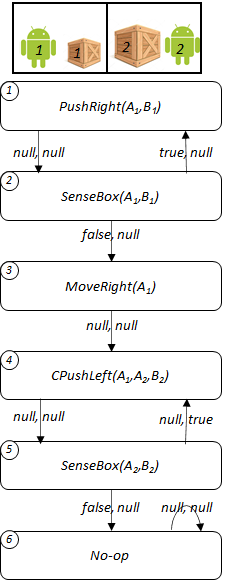
\includegraphics[scale=0.35]{pi.team.2.png}}
     \quad
     \subfloat[\label{fig:pi.tag.a1}$\pi'_1$]{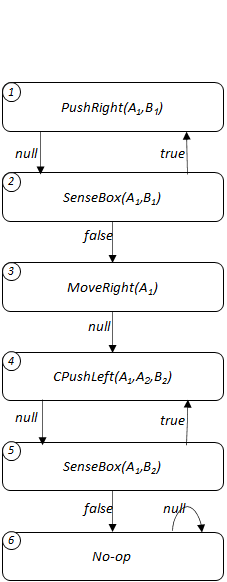
\includegraphics[scale=0.35]{pi.tag.a1.png}}
       \quad
    \subfloat[\label{fig:pi.a1}$\pi_1$]{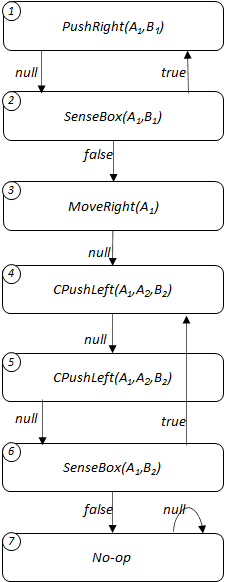
\includegraphics[scale=0.35]{pi.a1.png}}
       \quad     
       \subfloat[\label{fig:pi.tag.a2}$\pi'_2$]{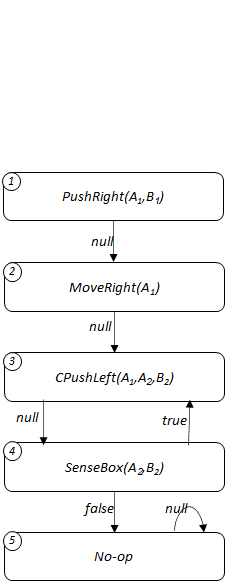
\includegraphics[scale=0.35]{pi.tag.a2.png}}
       \quad
     \subfloat[\label{fig:pi.a2}$\pi_2$]{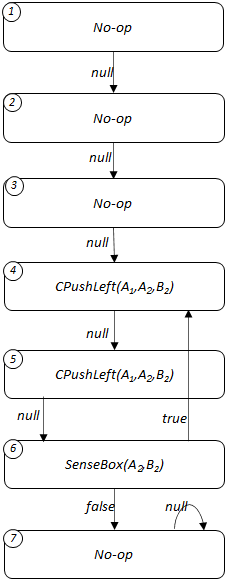
\includegraphics[scale=0.35]{pi.a2.png}}
 \caption{\label{fig:example} A 2-cell box pushing problem, and the resulting plan graphs. The agents must switch between the boxes. Box $B_1$ is light, $B_2$ is heavy and must be pushed by the two agents jointly.}
 \end{figure}

 \end{example}

\commentout{
\begin{figure}
    \centering
    \subfloat{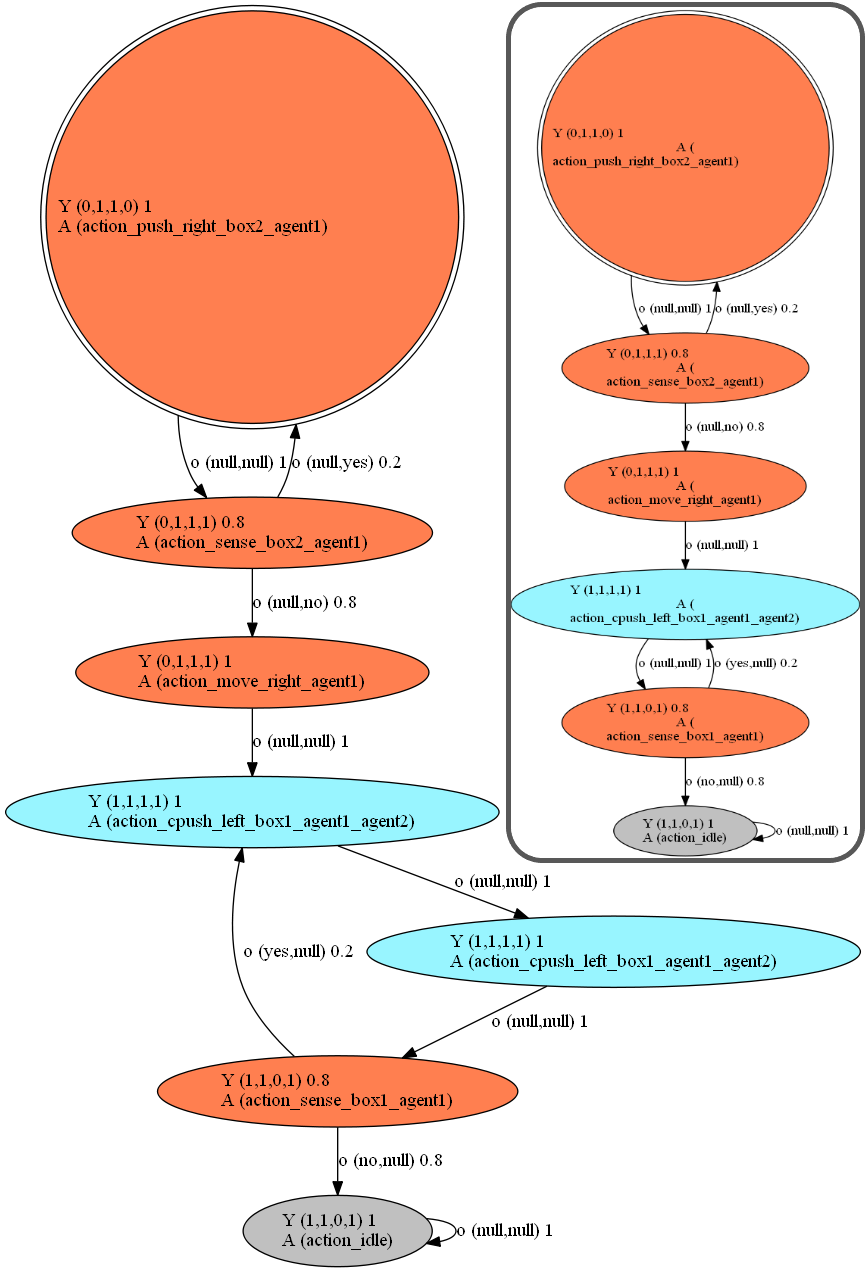
\includegraphics[width=0.39\textwidth,height=\textheight,keepaspectratio]{Agent1-Both-Graphs.png}}
\caption{\label{Fig:Alignment} $A_1$'s Policy, Before (framed) And After Alignment and Adjustments.}
\end{figure}
}
%\end{example}


\commentout{
\begin{algorithm}
\caption{Alignment Iteration}
\begin{algorithmic}[tbph]
\State Input: PolicyGraphs $G_1, \ldots, G_M$
\For{$G_i,  i\in\{1, \ldots, M\}$}
	\State {$\mathit{NoopsReqs} \gets \mathit{VertexToIntMapping}$}
      \State {$\mathit{CurrBFS} \gets \Call{BFS}{G_i}$}
      \While {$\mathit{CurrBFS.queue}$ is not empty}
	\State {$v \gets \mathit{CurrBFS.queue.pop}$}
	\State {$a \gets v.action$}
	\If {$a$ is public action}
	\State {$\mathit{identifier} \gets \Call{GetIdentifier}{v}$}
	\State {$\mathit{MaxNoop} \gets 0$}
	\For {$G_j,  j\in\{1, \ldots, M\}\setminus\{i\}$}
	\State {$\mathit{CurrNoop} \gets \Call{NoopReq}{G_j, \mathit{identifier}}$}
	\State {$\mathit{MaxNoop} \gets max(\mathit{MaxNoop}, \mathit{CurrNoop})$}
	\EndFor
	\State {$\mathit{NoopsReqs}[v] \gets \mathit{MaxNoop} - \mathit{CompensationTerm}$}
	\EndIf
	\EndWhile
	\State {$G_i' \gets \Call{AddNoops}{G_i, \mathit{NoopsReqs}}$}
\EndFor
\State {return $G_1', \ldots, G_M'$}
\end{algorithmic}
\end{algorithm}
}

\section{Empirical Evaluation}

We evaluate our algorithm 
on 3 domains: two variations of the popular cooperative Box Pushing, Dec-Tiger and Rock Sample. TIS uses SARSOP \citep{SARSOP} as the underlying POMDP solver.
%\subsection{Competitive Solvers}

We compare TIS, with 3 Dec-POMDP solvers, GMAA*-ICE \citep{GMAAICE}, JESP \citep{JESP}, 
and DICEPS~\cite{DICEPS} using MADP-tools \citep{MADP}.
The GMAA*-ICE solver provides optimality guarantees.
JESP searches in policy space, performing alternating maximizations using dynamic programming. DICEPS is an approximate method, which does not excel on smaller domains, but presumably can scale to larger domains.%
\footnote{DICEPS, while not new, was recommended to us, independently, by two senior researchers as still being a state-of-the-art approximate solver.}
%\footnote{Frans Oliehoek and Matthijs Spaan, personal communication.} 
We also compare TIS to 3 state-of-the-art MARL algorithms: 
two versions of WQMix~\cite{WQmix}, and QTRAN~\cite{Qtran}
%and CMAE~\cite{CMAE}.
%CW QMIX (centrally weighted) and OW QMIX (optimistically weighted) are MARL algorithms that are scalable versions of QMIX MARL algorithm.
%QTRAN is an MARL algorithm that is free from structural constraints and takes on a new approach to transforming the original joint action-value function into an easily factorizable one, with the same optimal actions.
%CMAE (cooperative multi agent exploration) is an MARL algorithm deals with the common challenge: agents struggle to identify states that are worth exploring, and hardly coordinate exploration efforts toward those states.
All experiments were conducted on a PC with Intel-core i7-5500U CPU @ 2.40GHz with 4 cores and 7.7GB of memory. TIS, GMMA-ICE, and JESP were run under Windows-11
and the others were run under Ubuntu 20.04.1.
%We run DICEPS, CW QMIX, OW QMIX, QTRAN, and CMAE on Ubuntu 20.04.1 machine running Intel-core i7-5500U CPU @ 2.40GHz with 4 cores and 7.7GB of memory.
% Below, we also discuss another approximate solver, described in~\citep{WuZJ13}, which was able to solve a huge 2d traffic domain.


%We also conducted a number of experiments using the state-of-the-art mutli-agent RL (MARL) algorithm CMAE~\cite{CMAE}. 

%MARL methods have demonstrated in the past few years an ability to tackle complex problems with large state spaces, requiring only a blackbox simulator of the domain rather than a complete formal model description. 

%Still, as we later demonstrate, MARL algorithms, while able to scale up to very large domains for which an explicit model is not available, are not competitive to Dec-POMDP solvers on domains that can be described efficiently using a formal model. As we show, MARL methods such as OW QMIX, CW QMIX, QTRAN, and CMAE require considerable more time than model-based methods on domains for which a model exists.
%(e2-standard-2 type in Google Cloud Platform). 

GMAA*-ICE and DP-JESP require an horizon specification, specified 
under column $H$. TIS computes a policy for an unbounded horizon and its
$H$-value specifies the average number of steps until reaching the goal state.
%under the column -Avg-. In some cases, instead of -Avg-, we specify the -H- column for TIS as well, which stands for the simulation length. 
 DICEPS uses restarts, and repeatedly returned an overflow error. To generate comparable running times to TIS, we rerun it multiple time, and used the maximal score over these runs, which is equivalent to simply letting it run longer. 

For GMAA*-ICE and DP-JESP we report the computed policy value. For TIS the {\em value} column provides the average discounted accumulated reward over 1000 simulations truncated at the relevant horizon. The {\em avg} column denotes average number of steps for all agents to reach the goal state.
For MARL algorithms, we measure maximum average discounted reward over a number of test runs.
The discount factor was set to $\gamma=0.99$.
%For CMAE MARL algorithm, we measure last average discounted reward of the test.

Planners were given 1 hour to solve each $\langle\textit{configuration, horizon}\rangle$ pair. MARL algorithms were given longer times. We report running times in seconds.
%Moreover, we set TIS with a limit of 900 seconds per agent. 

%The time shown for DP-JESP and GMAA*-ICE is based only on its log from the MADP-Toolbox, and does not include the problem loading, which is often non negligible. TIS time does not include writing the SARSOP policies and graphs to disk, as they are highly dependent on hardware quality and can effectively remain in memory.
\subsection{Domains}
{\bf \ \ Box Pushing:} agents on a grid must push boxes to their destinations \cite{carlin2008value,QDECPOMDP}. Light boxes can be pushed by a single agent. Heavy boxes must be pushed collaboratively by two agents. 
Agents can sense for a box at the present location. The initial box locations are uncertain. 
%Initially, each box can appear in either the target cell (and hence, need not be moved) or the lower right cell, with equal probability.
%The goal of the agents is to move the boxes to a target cell, located at the upper left corner of the grid.
%Action costs are: 10 for {\em Move}, 1 for sensing actions, 30 for {\em Push}, 20 (per agent) for {\em Collaborative Push} and 0 for {\em no-op}. The reward for moving a box to its target position is 500. In addition, there's a penalty of 10000 for pushing a box \emph{out} of the target cell to avoid abuse. For heavy boxes we double the reward and penalty. 
We also consider a variant of this domain in which we add a penalty when a push action is performed in a cell with
no box.
%, demonstrating certain differences between policies produced by different planners.
Problem names are composed of 5 elements, specifying
%specified in brackets, $\textit{BP}-W,H,n,l,h$. These elements denote
width, height, number of agents, number of light boxes, and number of heavy boxes.
% A domain instance of $m$ cells with $n$ agents, $l$ light boxes, and $h$ heavy boxes, has $m^{n+l+h}$ states, $(5\cdot(l+1)+4h\cdot(n-1))^n$ actions and $3^n$ observations.

% Evidently, the box pushing domain calls for longer horizon policies, rather than good local reactive policies, and requires careful coordination to ensure that collaborative push actions are performed simultaneously by the agents.

%\subsection{\cdt}
{\bf Dec-Tiger:} 
%We adapt the Dec-Tiger problem presented in \citep{JESP}. 
Agents must open a door avoiding a tiger \cite{nair2003taming}. The tiger's location resets following a door opening. Collaboratively opening a tiger door results in a lower penalty compared to single agent opening actions. Agents have noisy observations on the tiger's location. We use a larger Dec-Tiger version that requires agents to move on a grid \cite{amato2010optimizing}.

%Finally, we allow the agents to independently receive informative observations, as we don't handle collaborative sensing actions. 
%The reward function is 
%essentially the same - the agent pays 
%-1 for listening, -100 for opening the tiger door alone, and -25 for collaboratively opening the tiger door (0 for move and idle actions).  10 for either opening the prize door alone or collaboratively. 
%The domain favors collaboration in terms of the penalty.

%\subsection{\drs}
{\bf Decentralized Rock-Sample:}
%In this domain, %, described in Figure~\ref{Fig:DRS}, 
We suggest a new variant of Mars exploration problem \cite{smith2005point}, where two rovers move on a grid
that contains rocks that must be sampled . The grid is divided into overlapping control areas, one per rover. The rovers can move around the grid, sense the rocks' quality, which is initially unknown, and sample them. Agents are rewarded for sampling all the good rocks in their control area, but penalized directly for sampling a bad quality rock. Once a good quality rock is sampled, it turns bad. Rovers have a long range sensor, whose quality deteriorates with increased distance from the rock. 
%Its maximal sensing ability has 10\% error rate. The costs are 1 and 5 for sense and move actions, and 500 for sampling a bad rock is 500. The reward for sampling all good rocks in a control area is 750.
%We experiment with different grid sizes and rocks amounts. 
Problem names are composed of the grid size and the number of rocks.
%The problem name has the structure $\textit{DRS-n,r}$, where $n$ is the grid size, and $r$ is the number of rocks.

These problems call for solutions of different types.
%\ronen{why local/reacting? no reward for collaborative action, only penalty}
In \cdt, the problem resets after one of the doors is opened and so the planning horizon can be short, there are no interdependent actions (i.e., ones setting up conditions for the execution of others), but tight coordination in the execution of door opening actions is desirable.
\cbp\ rewards the agents for pushing a box to the target tile, requiring aggregating a chain of properly-directed pushes of a box to a single reward. With light boxes, a simple plan can use a single agent. Yet, efficient plans make use of the different agent positions to reduce (costly) move actions. With heavy boxes, agents must push the box at the same time, requiring even better coordination. The second box-pushing variant calls for trading off the cost of additional sensing with the penalty for moving a non-existent box.
%\ronen{Can some boxes be pushed by a single agent only?}
\drs\ rewards an agent only for achieving all of its objectives, which makes large-horizon planning ability crucial, giving no reward at all to partial solutions.

\commentout{
\begin{figure}[ht]
    \centering
    \subfloat{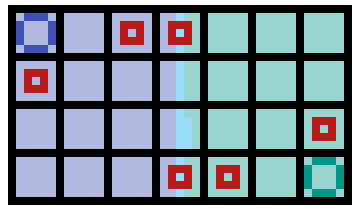
\includegraphics[width=0.35\textwidth,height=\textheight,keepaspectratio]{drsgrid.png}}
\caption{\label{Fig:DRS} \drs. The agents are located in the grid's corners.
Their corresponding control area is colored similarly. Rocks are the red squares, whose condition is unknown. The middle column is the shared zone.}
\end{figure}
}

\commentout{
%\subsection{Settings} 

GMAA*-ICE and DP-JESP require an horizon specification, while TIS computes a policy for an unbounded horizon. Therefore, we specify the maximal reached planning horizon for them under the column -H-, and for TIS we specify the average number of steps until reaching the goal state, under the column -Avg-. In some cases, instead of -Avg-, we specify the -H- column for TIS as well, which stands for the simulation length. Discount factor is set to $\gamma=0.99$. DICEPS uses restarts, and in the box pushing domain repeatedly returns an overflow error. Thus, to generate comparable running times to TIS in this domain, we rerun it multiple time, and used the maximal score over these runs, which should be equivalent to simply letting it run longer, if no errors were generated. 
%
For GMAA*-ICE and DP-JESP we report the computed policy value. For TIS we measured the average discounted accumulated reward over 1000 simulations. 

For OW QMIX, CW QMIX, and QTRAN MARL algorithms, we measure maximum average discounted reward of test.

%For CMAE MARL algorithm, we measure last average discounted reward of the test.

%
%We provide results on several configurations of \cbp, \drs , and the known configuration of \cdt.
\commentout{
In \cbp, each box starts at either the top-left or bottom-lower corner with equal probabilities. The problem name is composed of 5 elements specified in brackets, $\textit{BP}-[w][h][n][l][h]$. These
elements denote
Width, Height, Number of agents, Number of light boxes, and Number of heavy boxes.
% For 1 dimensional grids, DP-JESP and GMAA*-ICE were given a minimalistic version of the problem that does not include unnecessary actions | push and move for the up and down directions | to decrease the domain size.
We specify the agents' initial locations (denoted by $I$), as well as the domain size ($S$ and $A$), alongside the configuration name.

In \cdt, each agent starts in a known location, while the tiger location is unknown, and has equal probability for each side.

In \drs, the agents start at the bottom right and upper left corners, and the rocks at known locations depending on the grid size. We experiment with different grid widths and rocks amounts, specified in the domain name with two corresponding marks, $\textit{DRS-[w][r]}$.
}

All planners were given a total of 1 hour to solve each\\ $\langle\textit{configuration, horizon}\rangle$ pair. We report running times in seconds. Moreover, we set TIS with a limit of 900 seconds per agent. The time shown for DP-JESP and GMAA*-ICE is based only on its log from the MADP-Toolbox, and does not include the problem loading, which is often non negligible. TIS time does not include writing the SARSOP policies and graphs to disk, as they are highly dependent on hardware quality and can effectively remain in memory. %throughout the whole process - this can be solved using a RAM drive or RAM file system abstractions.

% In both GMAA*-ICE and DP-JESP, configurations BP-32302, BP-32303 and BP-33221 could not be solved for any horizon. Therefore we provide comparisons only for the first four configurations (Table \ref{tbl:scale}), while the harder configurations are shown in Table \ref{tbl:maxres}. We also provide a more sensitive analysis of the horizon in table \ref{tbl:small}

%In DP-JESP, $\times$ marks a timeout. In GMAA*-ICE we mark two different timeout options: FF refers to failure of finding a full policy for the required horizon, where FH refers to an earlier stage timeout when computing the heuristic function.
%\eliran{I want to remove the above paragraph since FH occurred only in the largest configurations, which I now centralized in a single table that doesn't even report the competing solvers' results. Is it ok? (FH is the more severe timeout, so it just acts in their favor).}

}



 \begin{table}[t]
 \centering
 \scriptsize
 \begin{tabular}{|c||c|c||c|c||c|c||c|c||c|c||c|c||c|c||}
         \hline
         \multicolumn{15}{|c|}{\cdt,  $|S|=8, |A|=5, I=\langle(0,1,0),(0,1,1)\rangle$} \\
         \hline
         H & \multicolumn{2}{|c||}{DP-JESP} & \multicolumn{2}{c||}{GMAA*-ICE} &
         \multicolumn{2}{c||}{DICESP} % & CMAE 
         & \multicolumn{2}{c||}{OW QMix} & \multicolumn{2}{c||}{CW QMix} & \multicolumn{2}{c||}{QTran} & \multicolumn{2}{c||}{TIS} \\
                  \hline
         \ & Time & Value & Time & Value & Time & Value % & 300 secs 
         & 300s & 3600s & 300s & 3600s & 300s &  3600s & Time & Value\\
         \hline
         3 & 0.42 & 1.96 & 0.24 & \textbf{11.15} & 121.54 & 0    % & 5.65 
         & -7.84 &  7.44  & -19.79 &   2.36  & 0 &  2.55 & 6.03 & 11.10 \\
         \hline
         4 & 33.15 & 10.05 & 841.67 & 11.03 & 155.98 & 3.2    % & -0.97  
         & -7.87 &  \textbf{13.602}  & 2.14 &  8.77  & 0 &  0.958 & " & 9.12 \\ 
         \hline
         5 & 1792.22 & 5.78 & $\times$ & - & 206.56 & 4.03   %&  7.87 
         & 1.68 &  \textbf{14.454}  & -1.82 &  12.93  & 0 &  4.08 & " & 8.56  \\
         \hline
         6 & $\times$ & - & $\times$ & - & 243.07 & 5    %& 12.85 
         & 2.61 & \textbf{15.473}  & -7.35 &  10.14  & 0 &  1.96 & "  & 9.05 \\
         \hline
          10 & $\times$ & - & $\times$ & -  & x & x    %&  2.09   
          & -17.79 &  \textbf{18.136}  & 6.31 &  11.59  & 0 &  0.758 & "  & 10.19\\
         \hline
          20 & $\times$ & - & $\times$ & -  & x & x     %& -4.47  
          & -13.91 &  \textbf{20.058}  & -2.79 &  12.84  & 0 &  1.79 & "  & 16.42 \\
         \hline
          30 & $\times$ & - & $\times$ & -  & x & x    %&  -3.1 
          & -19.43 &  18.954  & -17.95 &  25.63  & 0.58 &  \textbf{54.907} & "  & 20.10 \\
         \hline
          40 & $\times$ & - & $\times$ & -  & x & x   %&  -3.06 
          & -11.702 &  \textbf{26.128}  & 0 &  23.86  & 0 &  10.49 & "  & 24.62 \\
         \hline
         %Max & 33.15 & 10.05 (4) & \textbf{0.24} & 11.15 (3) & 6.63 & \textbf{29.25} (49) \\
         %\hline
    \end{tabular}
    
    \caption{\label{tbl:scale_CDT} Results for \cdt\ on state-of-the-art Dec-POMDP and MARL solvers and TIS. Best overall value for each problem in bold.
    %TIS manages to obtain competitive results on small horizons, while demonstrating a consistent value improvement in larger horizons.
    }
    \vspace{-4mm}
\end{table}


\commentout{
 \begin{table*}[t]
 \centering
 \footnotesize
 \begin{tabular}{|c||c|c||c|c||c|c||}
         \hline
         \multicolumn{7}{|c|}{\cdt,  $|S|=8, |A|=5, I=\langle(0,1,0),(0,1,1)\rangle$} \\
         \hline
         H & 
         \multicolumn{2}{|c||}{OW QMIX} & 
         \multicolumn{2}{c||}{CW QMIX} &
         \multicolumn{2}{c|}{QTRAN} &
         \hline
         & Time & Value & Time & Value & Time & Value \\
         \hline 3 & 3600 & 7.44 & 3600 & 2.36 & 3600 & 2.55 \\ 
         \hline 4 & 3600 & \textbf{13.602} & 3600 & 8.77 & 3600 & 0.958 \\ 
         \hline 5 & 3600 & \textbf{14.454} & 3600 & 12.93 & 3600 & 4.08 \\ 
         \hline 6 & 3600 & \textbf{15.473} & 3600 & 10.14 & 3600 & 1.96 \\ 
         \hline 10 & 3600 & \textbf{18.136} & 3600 & 11.59 & 3600 & 0.758 \\ 
         \hline 20 & 3600 & \textbf{20.058} & 3600 & 12.84 & 3600 & 1.79 \\ 
         \hline 30 & 3600 & 18.954 & 3600 & 25.63 & 3600 & \textbf{54.907} \\ 
         \hline 40 & 3600 & \textbf{26.128} & 3600 & 23.86 & 3600 & 10.49 \\ 
        \hline
         %Max & 33.15 & 10.05 (4) & \textbf{0.24} & 11.15 (3) & 6.63 & \textbf{29.25} (49) \\
         %\hline
    \end{tabular}
    
    \caption{\label{tbl:scale_CDT} Results for \cdt, on state-of-the-art MARL algorithms. 
    %TIS manages to obtain competitive results on small horizons, while demonstrating a consistent value improvement in larger horizons.
    }
\end{table*}
}



\begin{table}[t]
\centering
    %\resizebox{\columnwidth}{!}{
    \scriptsize
    \begin{tabular}{|c|c|c||c|c|c||c|c|c||c|c|c||c|c|c||}
         \hline
          \multicolumn{15}{|c|}{\cbp} \\
         \hline
         \multicolumn{3}{|c||}{Problem} &\multicolumn{3}{|c||}{DP-JESP} & \multicolumn{3}{c||}{GMAA*-ICE} & \multicolumn{3}{|c||}{DICEPS} & \multicolumn{3}{c||}{TIS} \\
         \hline
         Name&$|S|$ & $|A|$ & H & Time & Value & H & Time & Value & H & Time & Value & Avg & Time & Value\\
         \hline\hline
        
         1: 3,1,2,1,1&81&16& 4 & 1861.30 & 279 & 4 & 30.23 & 330.07 & 4 & 221.71 & 0 & 15 & 6.07 & 613.98  \\
         
         \hline
         
 
         2: 2,2,2,0,2&256 & 225   &3 & 267.24 & 271 & 3 & 160.18 & 320.46 & 3  & 348.56 & 0 & 9 & 7.08 & \textbf{348.56} \\
         \hline
         
         
         
         \hline
         3: 2,2,2,0,3& 1024 & 400  &2 & 59.06 & 0 & 2 & 1053.27 & 414 & 2 & 514.09 & 0 & 17 & 125.50 & \textbf{514.09}  \\
         \hline
         1-Penalty &81&16& 3 & 25.95 & 0 & 4 & 79.28 & 265.44 & - & - & - 
         & 15 & 8.54 & 586.96 \\
         \hline 

         2-Penalty &256 & 225 & 3 & 495.61 & 135.40 & 3 & 446.03 & 213.79  & - & - & -  &  9 & 11.66 & \textbf{354.29} \\
         \hline 
         
         3-Penalty & 1024 & 400 & 2 & 38.70 & 0 & 2 & 1054.5 & 326.50 & - & - & -  & 15 & 31.09 & \textbf{510.13}  \\
         
         
         \hline
                  \hline
                  
        \multicolumn{3}{|c||}{} &\multicolumn{3}{|c||}{OW QMIX} & \multicolumn{3}{c||}{CW QMIX} & \multicolumn{3}{c||}{QTRAN} & \multicolumn{3}{c||}{TIS}\\

         \hline 
        \multicolumn{3}{|c||}{} & H & 300s & 7200s & H & 300s & 7200s & H & 300s & 7200s & Avg & Time & Value\\
         \hline
         1: 3,1,2,1,1&81&16 & 20 & 120.27 & 1165.318 & 20 & -8.91 & \textbf{1177.25} & 20 & 345.17 & 348.42  & 15 & 6.07 & {\bf 613.98} \\
         
         \hline
         
         2: 2,2,2,0,2&256 & 225    & 15 & -3.57 & -1.98 & 15 & 0 & 0 & 15 & 0 & -0.79 & 9 & 7.08 & \textbf{348.56} \\
         \hline
         
         
         3: 2,2,2,0,3& 1024 & 400  & 20 & -2 & 0 & 20 & 0 & -2 & 20 & -0.8 & 0 & 17 & 125.50 & \textbf{514.09}\\
         \hline
         
         1-Penalty &81&16& 20 & -36.32 & 1143.856& 20 & 76.97 & \textbf{1190.74} & 20 & -77.94 & 371.54
         & 15 & 8.54 & {\bf 586.96} \\
         \hline 
         
         2-Penalty &256 & 225  & 15 & 0 & -3.9  & 15& 0 & 0  & 15& 0 & 0 & 9 & 11.66 & \textbf{354.29} \\
         \hline 
         

         3-Penalty & 1024 & 400   & 20 & 0 & 0 & 20& 0 &  0 & 20 & -35.62 &  -29.34  & 15 & 31.09 & \textbf{510.13}  \\
         \hline 

         3,2,3,0,2 &
         $7776$& $3375$   & 20 & 0 & 0  & 20 & 0 & - & 20 & 0  & 0 & 12 & 89.83 & {\bf 275.76} (100)\\
          
         \hline
         3,2,3,0,3 &
         $46656$ & $8000$   &20 & 0 & 0 & 20 & 0 & 0 & 20 & 0 & 0 & 18 & 2210.28 & {\bf 406.22} (100) \\
         
         \hline
%         3,3,2,2,1 &
%         $59049$&$324$     & -2 & 0  & 0   & 43 & 2863.08 & \textbf{125.23} & 99\\
         
         \hline
         3,3,2,2,1 &
         $59049$&$324$     &20 & -4.37 & -2 & 20 & 0 & 0 & 20 & -72.76 & 0 & 39 & 3014.04 & {\bf 321.81} (100) \\
                 \hline
         
         \hline

                  \hline
        
        
         \multicolumn{15}{|c|}{\drs} \\
         \hline
         \multicolumn{3}{|c||}{Problem} &\multicolumn{3}{|c||}{DP-JESP} & \multicolumn{3}{c||}{GMAA*-ICE} & \multicolumn{3}{|c||}{DICEPS} & \multicolumn{3}{c||}{TIS}\\
        
        \hline
         12,3 & 512 & 90    & 3 & 314.35 & 224.38 & 3 & 82.86 & 738.88 & 3 &  2018 & 755 & 18 & 1725.80 & \textbf{1027.88} \\
         
         \hline
      
         
         12,4 & 1024 & 100 & 3 & 1081.41 & 518.19 & 3 & 2867.06 & 507.76 & 3 & 2763 & 495 & 20 & 2438.82 & \textbf{1048.11}  \\
         
         \hline
       
         
         20,4 & 2304 & 100  & 3 & 1838.84 & 111.25 & 3 & - & -  & 3 & 2868 & 514 & 16 & 2434.88 & \textbf{1157.95} \\
         \hline \hline
         
         \multicolumn{3}{|c||}{} &\multicolumn{3}{|c||}{OW QMIX} & \multicolumn{3}{c||}{CW QMIX} & \multicolumn{3}{c||}{QTRAN} & \multicolumn{3}{c||}{TIS}\\
         \hline
         \multicolumn{3}{|c||}{} & H & 300s & 7200s & H & 300s & 7200s & H & 300s & 7200s & Avg & Time & Value\\
         \hline
         12,3 & 512 & 90  & 25 & -56.51 & 473.6369 & 25 & -54.42 & 508.85 & 25 & -34.28 & 608.91 & 18 & 1725.80 & \textbf{1027.88}\\
         
         \hline
         %H & Time & Value & H & Time & Value & Avg & Time & Value \\
         
         12,4 & 1024 & 100  & 25 & -45.6 & 198.122 & 25 & -12.00 & 202.905 & 25 & 0 & 616.86 & 20 & 2438.82 & \textbf{1048.11}\\
         
         \hline
         %H & Time & Value & H & Time & Value & Avg & Time & Value \\
         
         20,4 & 2304 & 100   & 25 & -55.20 & 451.725 & 25 & -45.63 & 219.45 & 25 & -40.05 & 327.19 & 16 & 2434.88 & \textbf{1157.95}\\
         \hline
         
         20,6 &
         $9216$&$143$  &25 &-19.34  & 134.86 &25& -43.85 & 19.83 &25& -21.83 & 407.76 & 21 & 2537.10 & \textbf{1121.12} (97) \\
         
         \hline
         28,6 &
         $16384$& 143   &25&-29.23 & 47.4 &25& 91.78 & 24.48 &25 & -1.99 & 0  & 23 & 3310.95 & \textbf{1045.74} (97)\\
         \hline
         
    \end{tabular}
    %}
    
    \caption{\label{tbl:scaleBP_DRS}
    %TIS outperforms DP-JESP and GMAA*-ICE with respect to policy value in both domains, and also with respect to running time in Box-Pushing. 
    TIS vs. Dec-POMDP solvers and vs. MARL solvers on Box-Pushing (BP) and Rock-Sample (DRS). Best  value per problem in bold.
    %Results for DP-JESP and GMAA*-ICE are for maximal horizon reached (-H- column). For TIS we present the average number of steps until reaching the goal state when running the policy for an unbounded number of steps, specified under the -Avg- column.
    }
    \vspace{-4mm}
\end{table}

\commentout{
\begin{table*}[t]
\centering
    %\resizebox{\columnwidth}{!}{
    \footnotesize
    \begin{tabular}{|c|c|c|c||c|c|c||c|c|c||c|c|c|}
         \hline
         \multicolumn{4}{|c||}{Problem} &\multicolumn{3}{|c||}{OW QMIX} & \multicolumn{3}{c||}{CW QMIX} & \multicolumn{3}{c||}{QTRAN} \\
         \hline
         Name&$|S|$ & $|A|$ & $I$ & H & Time & Value & H & Time & Value & H & Time & Value  \\
         % & H & Time & Value \\
         \hline\hline
         \multicolumn{13}{|c|}{\cbp} \\
         \hline
         3,1,2,1,1&81&16& $\langle(1,2),(1,3)\rangle$ & 20 & 7200 & 1165.318 & 20 & 7200 & \textbf{1177.25} & 20 & 7200 & 348.42 \\ % & 4 & 221.71 & 0 \\
         
         \hline
         
         2,2,2,0,2&256 & 225 & $\langle(1,2),(2,2)\rangle$   & 15 & 7200 & -1.98 & 15 & 7200 & 0 & 15 & 7200 & -0.79 \\ % & 3 & 348.56 & 0 \\
         \hline
         
         
         2,2,2,0,3& 1024 & 400 & $\langle(1,2),(2,2)\rangle$ & 20 & 7200 & 0 & 20 & 7200 & -2 & 20 & 7200 & 0 \\ % & 2 & 514.09 & 0  \\
         \hline
                  \hline
         \multicolumn{13}{|c|}{\drs} \\
         \hline
         %H & Time & Value & H & Time & Value & Avg & Time & Value \\
        
         12,3 & 512 & 90 & $\times$  & 25 & 7200 & 473.6369 & 25 & 7200 & 508.85 & 25 & 7200 & 608.91 \\ % & 3 &  2018 & 755  \\
         
         \hline
         %H & Time & Value & H & Time & Value & Avg & Time & Value \\
         
         12,4 & 1024 & 100 & $\times$ & 25 & 7200 & 198.122 & 25 & 7200 & 202.905 & 25 & 7200 & 616.86 \\ % & 3 & 2763 & 495  \\
         
         \hline
         %H & Time & Value & H & Time & Value & Avg & Time & Value \\
         
         20,4 & 2304 & 100 & $\times$  & 25 & 7200 & 451.725 & 25 & 7200 & 219.45 & 25 & 7200 & 327.19 \\
         \hline
         
    \end{tabular}
    %}
    
    \caption{\label{tbl:scaleBP_DRS}
    %TIS outperforms DP-JESP and GMAA*-ICE with respect to policy value in both domains, and also with respect to running time in Box-Pushing. 
    Scaling up in Box-Pushing (BP) and Rock-Sample (DRS), on state-of-the-art MARL algorithms.
    %Results for DP-JESP and GMAA*-ICE are for maximal horizon reached (-H- column). For TIS we present the average number of steps until reaching the goal state when running the policy for an unbounded number of steps, specified under the -Avg- column.
    }
\end{table*}
}

\commentout{
\begin{table*}[t]
\centering
\footnotesize
    %\resizebox{\columnwidth}{!}{
    % Our policy graph's longest Hamiltonian path is of length 12 - this implies that a maintainable coordination was found, which does not break after a single cycle.}
        \begin{tabular}{|c|c|c|c|c|c|c||c|c|c|c|c||c|c|c|}
         \hline
         \  &\multicolumn{3}{|c|}{DP-JESP} & \multicolumn{3}{c|}{GMAA*-ICE} & \multicolumn{2}{|c|}{MARL H/T} & OW QMIX & CW QMIX & QTRAN & \multicolumn{3}{c||}{TIS}\\
         \hline
         Prob. & H & Time & Value & H & Time & Value &  H & Time & Value & Value &  Value & Avg & Time & Value \\
         \hline
         1  & 3 & 25.95 & 0 & 4 & 79.28 & 265.44 & 20 & 7200 & 1143.856  & \textbf{1190.74} & 371.54 & 15 & 8.54 & 586.96 \\
         \hline
         2  & 3 & 495.61 & 135.40 & 3 & 446.03 & 213.79  & 15 & 7200 & -3.9   & 0   & 0 & 9 & 11.66 & \textbf{354.29} \\
         \hline
         3  & 2 & 38.70 & 0 & 2 & 1054.5 & 326.50 & 20 & 7200 & 0 &   0 &   -29.34 & 15 & 31.09 & \textbf{510.13}  \\
         \hline
    \end{tabular}
    %}
    
    \caption{\label{tbl:bppen} Results for \cbp\ with extra penalty for pushing a non-existent box}\end{table*}
}

\commentout{

\begin{table*}[t]
\centering
\footnotesize
    %\resizebox{\columnwidth}{!}{
    % Our policy graph's longest Hamiltonian path is of length 12 - this implies that a maintainable coordination was found, which does not break after a single cycle.}
        \begin{tabular}{|c|c|c|c||c|c|c||c|c|c||c|c|c|}
         \hline
         \multicolumn{4}{|c||}{Problem} &\multicolumn{3}{|c||}{OW QMIX} & \multicolumn{3}{c||}{CW QMIX} & \multicolumn{3}{c|}{QTRAN}\\
         \hline
         Name & $|S|$ & $|A|$ & $I$ & H & Time & Value & H & Time & Value & Avg & Time & Value \\
         \hline
         3,1,2,1,1 & 81 & 16 & $\langle(1,2),(1,3)\rangle$ & 20 & 7200 & 1143.856 & 20 & 7200 & \textbf{1190.74} & 20 & 7200 & 371.54 \\
         \hline
         2,2,2,0,2 & 256 & 225 & $\langle(1,2),(2,2)\rangle$    & 15 & 7200 & -3.9 & 15 & 7200 & 0 & 15 & 7200 & 0 \\
         \hline
         2,2,2,0,3 & 1024 & 400 & $\langle(1,2),(2,2)\rangle$        & 20 & 7200 & 0 & 20 & 7200 & 0 & 20 & 7200 & -29.34 \\
         \hline
    \end{tabular}
    %}
    
    \caption{\label{tbl:bppen} Results for \cbp\ with extra penalty for pushing a non-existent box, on state-of-the-art MARL algorithms.}
\end{table*}
}

\commentout{
\begin{table*}[t]
\centering
\footnotesize
    %\resizebox{\columnwidth}{!}{
    %\vspace{-20em}
    \begin{tabular}{|c|c|c||c|c|c||c|c|c|c|}
         \hline
         \multicolumn{3}{|c||}{Problem} &OW QMIX & CW QMIX & QTRAN &\multicolumn{4}{c|}{TIS}\\ 
         \hline
         Name & $|S|$ & $|A|$   & Value & Value & Value  & AvgSteps & Time & Value & \%Wins \\
         \hline
         \multicolumn{10}{|c|}{\cbp\ }\\
         \hline
         3,2,3,0,2 &
         $7776$& $3375$   & \ & \ & \ & 12 & 89.83 & 275.76 & 100\\
          
         \hline
         3,2,3,0,3 &
         $46656$ & $8000$    & \ & \ & \ & 18 & 2210.28 & 406.22 & 100 \\
         
         \hline
         3,3,2,2,1 &
         $59049$&$324$     & -2 & 0  & 0   & 43 & 2863.08 & \textbf{125.23} & 99\\
         
         \hline
         3,3,2,2,1* &
         $59049$&$324$     & not applicable  & not applicable & not applicable & 39 & 3014.04 & 321.81 & 100 \\
                 \hline
         \multicolumn{10}{|c|}{\drs\ }\\

         \hline
         20,6 &
         $9216$&$143$    & 134.86 & 19.83 & 407.76 & 21 & 2537.10 & \textbf{1121.12} & 97 \\
         
         \hline
         28,6 &
         $16384$& 143    & 47.4 & 24.48 & 0  & 23 & 3310.95 & \textbf{1045.74} & 97\\
         \hline
    \end{tabular}
    %}
    
    \caption{\label{tbl:maxres} Results for the larger problems.
    %-- solvable by TIS and state-of-the-art MARL algorithms only, on TIS. %Running times are rapidly increasing while reaching the scales limit of the underlying POMDP solver. The policies are still very robust, and reach the goal state in most cases (\%Wins). 
    %MaxSteps and AvgSteps specify the maximal and average number of steps made until reaching a goal state throughout the runs. 
    *: Limit of 1800 sec. per agent.}
    
\end{table*}
} 

\commentout{
\begin{table*}[t]
\centering
\footnotesize
    %\resizebox{\columnwidth}{!}{
    %\vspace{-20em}
    \begin{tabular}{|c|c|c|c||c|c|c|c|c|c|}
         \hline
         \multicolumn{4}{|c||}{Problem}&\multicolumn{5}{c|}{TIS}\\ 
         \hline
         Name & $|S|$ & $|A|$ & Initial positions & MaxSteps & AvgSteps & Time & Value & \%Wins\\
         \hline
         \multicolumn{9}{|c|}{\cbp\ }\\
         \hline
         3,2,3,0,2 &
         $7776$& $3375$b& $\langle(1,2),(1,3),(2,3)\rangle$ & 31 & 12 & 89.83 & 275.76 & 100 \\
          
         \hline
         3,2,3,0,3 &
         $46656$ & $8000$ &$\langle(1,2),(1,3),(2,3)\rangle$ &  45 & 18 & 2210.28 & 406.22 & 100 \\
         
         \hline
         3,3,2,2,1 &
         $59049$&$324$ &$\langle(1,3),(3,1)\rangle$ &  110 & 43 & 2863.08 & \textbf{125.23} & 99 \\
         
         \hline
         3,3,2,2,1* &
         $59049$&$324$ &$\langle(1,3),(3,1)\rangle$  & 121 & 39 & 3014.04 & 321.81 & 100 \\
                 \hline
         \multicolumn{9}{|c|}{\drs\ }\\

         \hline
         20,6 &
         $9216$&$143$ & & 33 & 21 & 2537.10 & \textbf{1121.12} & 97\\
         
         \hline
         28,6 &
         $16384$&$=143$ & & 38 & 23 & 3310.95 & \textbf{1045.74} & 97 \\
         \hline
    \end{tabular}
    %}
    
    \caption{\label{tbl:maxres} Results for the largest problems -- solvable by TIS and state-of-the-art MARL algorithms only, on TIS. %Running times are rapidly increasing while reaching the scales limit of the underlying POMDP solver. The policies are still very robust, and reach the goal state in most cases (\%Wins). 
    MaxSteps and AvgSteps specify the maximal and average number of steps made until reaching a goal state throughout the runs. *: 1800 sec. per agent.}
    
\end{table*}



\begin{table*}[t]
\centering
\footnotesize
    %\resizebox{\columnwidth}{!}{
    %\vspace{-20em}
    \begin{tabular}{|c|c|c|c||c|c|c||c|c|c||c|c|c|}
         \hline
         \multicolumn{4}{|c||}{Problem} & \multicolumn{3}{c|}{OW QMIX} & 
         \multicolumn{3}{c|}{CW QMIX} &
         \multicolumn{3}{c|}{QTRAN}
         \\ 
         \hline
         Name & $|S|$ & $|A|$ & Initial positions & H & Time & Value & H & Time & Value & H & Time & Value  \\
         \hline
         \multicolumn{13}{|c|}{\cbp\ }\\
         %\hline
         %3,2,3,0,2 &
         %$7776$& $3375$b& $\langle(1,2),(1,3),(2,3)\rangle$ & 31 & 12 & 89.83 & 275.76 & 100 \\
          
         %\hline
         %3,2,3,0,3 &
         %$46656$ & $8000$ &$\langle(1,2),(1,3),(2,3)\rangle$ &  45 & 18 & 2210.28 & 406.22 & 100 \\
         
         \hline
         3,3,2,2,1 &
         $59049$&$324$ &$\langle(1,3),(3,1)\rangle$ & 45 & 7200 & -2 & 45 & 7200 & 0 & 45 & 7200 & 0 \\
         
         \hline
         %3,3,2,2,1* &
         %$59049$&$324$ &$\langle(1,3),(3,1)\rangle$  & 121 & 39 & 3014.04 & 321.81 & 100 \\
                 %\hline
         \multicolumn{13}{|c|}{\drs\ }\\

         \hline
         20,6 &
         $9216$&$143$ & & 25 & 7200 & 134.863 & 25 & 7200 & 19.83 & 25 & 7200 & 407.76 \\
         
         \hline
         28,6 &
         $16384$&$=143$ & & 25 & 7200 & 47.397 & 25 & 7200 & 27.48 & 25 & 7200 & 0 \\
         \hline
    \end{tabular}
    %}
    
    \caption{\label{tbl:maxres} Results for the largest problems -- solvable by TIS and state-of-the-art MARL algorithms only, on state-of-the-art MARL algorithms. %Running times are rapidly increasing while reaching the scales limit of the underlying POMDP solver. The policies are still very robust, and reach the goal state in most cases (\%Wins). 
   }
    
\end{table*}
}


%Results are presented in Tables \ref{tbl:scale}, \ref{tbl:dt}. These problems call for solutions of different types. \cdt\ rewards or penalizes the agent for any single move, requiring local and reactive planners. Next comes \cbp, which rewards the agents for pushing a box to the target tile, aggregating a chain of well-directed pushes of a box to a single reward. Finally, \drs\ rewards an agent only for achieving all of its objectives, which makes large-horizon planning ability crucial, giving no reward at all to partial solution.

%\ronen{don't understand the above. seems like you are repeating the properties of the domains}\eliran{I see we only stated it previously in the end of 4.1. I think this would be a good place to present them, since our conclusions are drawn based on these properties. Should we remove it from 4.1?}
%\ronen{yes. no point of repeating in the same section}\eliran{I removed it from 4.1 then, it appears only here now.}

\subsection{Results}

Table~\ref{tbl:scale_CDT} describes the results for Dec-Tiger.
%), which is a well known benchmark for Dec-POMDP solvers. As other algorithms require the horizon as input, we report results over a growing horizon. 
GMAA*-ICE, which is an optimal solver, produces the best policy for the shortest horizon, but cannot scale beyond 4 steps. JESP scales to horizon 5, and DICEPS to horizon 6, but they produce policies of much lower quality than TIS, which can handle horizon 40 in about 6 seconds. DICESP, which should be able to scale well, terminated with an error after roughly 10-20 seconds for horizons 10 and higher. 
For the MARL algorithms we show results for two running times: 300 and 3600 seconds.
In this domain, OW-QMix was able to perform better than TIS, but only
when given 3600 seconds, as opposed to 6 for TIS. In the horizon 30 case, QTran was able to perform much better than TIS, but performed far worse on other horizons. Except for this case, TIS performed comparatively to,
or better than other MARL algorithms but required much less time. As can be seen from the results for 300 seconds, MARL algorithms cannot compete with
TIS as far a policy quality with shorter running times, even when
given 50X running time. 

%We also ran CMAE on \cdt. As CMAE is an anytime algorithm, we stopped it at different time intervals to evaluate its policy. As can be seen, the performance of CMAE is non-monotone with respect to time and horizon. CMAE may find the best policy for horizon 5 after 300 seconds, 50 times longer than TIS, but the policy for horizon 4 after this amount of time is non-competitive. For horizon 4, CMAE finds a good policy after 60 seconds, but fails to find a policy after 300 seconds.

%We also compare TIS to three state-of-the-art MARL algorithms: OW QMIX, CW QMIX, and QTRAN.
%On horizon 3, TIS scores better than all the state-of-the-art MARL algorithms. But on horizons larger than 3, QMIX variants scores better than TIS and TIS scores better than QTRAN. All those state-of-the-art MARL algorithms require much more time (7200 seconds) than TIS (6.05 seconds) to give those results.

Table~\ref{tbl:scaleBP_DRS} 
shows results for Box Pushing and Rock Sample. Both DP-JESP and GMAA*-ICE could not handle horizons larger than 3, while TIS can consider much longer action sequences, and, as such, collect much higher rewards. As noted above, \drs\ requires much lengthier horizons to achieve any reward, and TIS's advantage here is pretty clear.
Among the MARL algorithms, QMix was able to produce much better results on one problem instance (again, requiring orders of magnitude more time), but MARL solvers failed on harder Box Pushing domains that contain more heavy boxes that require a collaborative push action. Similar results were obtained with the alternative reward function, punishing attempts to push a non-existent box.
TIS is consistently better and faster than the MARL solvers on Rock Sample, again due to MARL difficulty in learning policies that require more complex coordination.

%TIS requires much more time in \drs\ compared to problems of similar scale in \cbp. This is because in box-pushing there is less uncertainty, as there are less boxes with unknown positions than rocks with unknown good-bad state. The higher the uncertainty, the more difficult it is to solve the generated POMDPs.

%CMAE on box pushing produced a policy with value $129.57$ on the smallest instance of box pushing (3,1,2,1,1) after 600 seconds, and failed to produce any reasonable policy on the larger instances. For \drs, with 3600 seconds, CMAE did not find any reasonable policy for any of the problems.


In the Box Pushing and Rock Sample we can also test the scalability of TIS.
These are domains  that current Dec-POMDP solvers cannot handle, and
hence we only provide a comparison with MARL algorithms. 
As can be seen, TIS can consider very long horizons even in these significantly larger problems. The size of the hardest configuration, BP-33221, approaches the maximal problems that the single agent POMDP solver SARSOP can solve, indicating that TIS could scale to even larger problems given a stronger POMDP solver. 
We are not aware of any other Dec-POMDP solver that is able to approach state sizes  even close to these on these domains: over 59000 in Box Pushing and over 16000 in Rock Sample. The MARL solvers were unable to generate reasonable solution within 7200 seconds for these larger problems. (For this reason, we do not 
provide results for shorter running times). 
%We note that we did not test CMAE on these domains since
To get a better grip of the meaning of the results on these domains, in the case of TIS we provide, in parenthesis, the percentage of successful trials. As can be seen, TIS's policy is able to achieve the goal in 100\% of the trials for Box Pushing and 97\% of the trials for Rock Sample. 



\begin{table}[t]
\centering
\scriptsize
    %\resizebox{\columnwidth}{!}{
    \begin{tabular}{|c||c|c||c|c|}
         \hline
          &  \multicolumn{2}{c||}{GMAA*-ICE} & \multicolumn{2}{c|}{TIS}\\ 
         \hline
         H & Time & Value & Time & Value \\
         \hline
         4  & 1.15 & \textbf{426.91} & 3.40 & 306.62 \\
         \hline
         5  & 2.09 & {\bf 438.34} & " & 301.56 \\ 
         \hline
         6 & 6.97 & {\bf 448.19} & " & 357.44 \\
         \hline
         7  & 8.98 & {\bf 450.97} & " & 412.54 \\
         \hline
         Max  & 17.1 & \textbf{454.70} (25) & 3.40 & 412.54 (7) \\
         \hline
    \end{tabular}
    %}
    
    \caption{\label{tbl:small} Comparing to optimal on small
    box pushing with $|S|=8$ and $|A|=16$. {\em Max} row is for maximal value for any horizon. ArgMax Horizon in parenthesis.
    }
    \vspace{-4mm}
\end{table}


%To observe the difference between the policies TIS produces to the ones GMAA*-ICE computes, we consider a variant of \cbp, where we add a penalty to push actions (for light boxes) that are executed with no box in the cell. Table~\ref{tbl:bppen} presents the results for this variant. We can see that the reward difference on maximal results compared to Table~\ref{tbl:scaleBP_DRS} are much lower for TIS, indicating that TIS creates policies, even in the non-penalized configurations, that exploit the horizon and favors sensing over blind pushing, leading to higher-quality results.

%On box-pushing and rock-sampling domains, we also compare TIS to three state-of-the-art MARL algorithms: OW QMIX, CW QMIX, and QTRAN.
%On box-pushing domains, both variants of QMIX score better than TIS on configuration 31211 with only 1 heavy box, that requires minimal agents cooperation. On rest of box-pushing domains, where more demanding agents cooperation required, on configuration with more than 1 heavy box, TIS gives the best scores.
%On rock-sampling domain, TIS also gives the best scores. We gave the state-of-the-art MARL algorithms 7200 seconds as a running time, much more time than the running time of TIS for box-pushing, and significantly more time than TIS requires in rock-sampling domains.

%\ronen{What "manages to reduce"?}\eliran{reformulated, should we elaborate on that? It seems that this number (of uncertain components) affects the running time much more than the sheer number of states. It's of course directly related to the underlying POMDP solver, which takes most of the computation time.}

TIS contains many heuristic choices that may cause it to obtain sub-optimal policies. To measure this, Table~\ref{tbl:small} focuses on a small box pushing problem that GMAA*-ICE can solve optimally. We see that TIS manages to produce reasonable results that are about 10\% worse on the larger horizons. Furthermore, in Dec-Tiger, which calls for strong agent synchronization, TIS does virtually 
the same as GMAA*-ICE on horizon 3. On medium size horizons TIS performs worse, probably because there is more opportunity for unsynchronized actions.

\subsection{Discussion}

As we  observed above, over the 3 domains that we experiment with, TIS is substantially better than all other solvers. It produces policies which are close to optimal on smaller problems with shorter horizons, and scales many orders of magnitude beyond existing Dec-POMDP solvers. 
%The methods that we compare against are a decade old, but no newer methods exist to compare against.

In comparison to state-of-the-art  MARL algorithms, TIS is much faster, and often returns much better policies. Of course, MARL algorithms do not receive the model as input and must compensate for it by running many trials. Nevertheless, we provide this comparison for two reasons. First, there is a perception that RL algorithms are a magic bullet and are the state-of-the-art for stochastic sequential decision making. Second, 
model-free RL algorithms are often suggested as an alternative to model-based solvers on domains with large state spaces, as they do not need to maintain and query an explicit model, which in larger problems can be difficult to represent. While this is certainly true, the time and resources required to compensate for the lack of a model can be substantial. 
As we have shown here,  domains that require better coordination
are still challenging for state-of-the-art MARL solvers. In longer (non-exhaustive) experiments conducted on QMIX, the results on these domains did not improve even given over 10 hours. Thus, we think that it can be safely concluded that when a model is available and a plan is needed quickly, TIS is currently the best
option.
%was not able to return gon the case of MARL algorithmsOn the other hand, there are real-world problems of interest, especially ones involving task planning, whose essence can be efficiently described by standard Dec-POMDP models. As we demonstrated above, our model-based solver can solve these problem faster and better than those MARL algorithms. In our experiment we stopped the state-of-the-art MARL algorithms after orders of magnitude more time that TIS required. Still, it is possible that given sufficient time, those MARL algorithms would have eventually found a solution.


Finally, we briefly discuss the MCEM Dec-POMDP solver~\cite{WuZJ13}. This algorithm is an example of an
approximate solver that can scale to huge problems. Indeed, MCEM was able to solve a grid-based traffic problem with 2500 agents and roughly $10^{100}$ states, which is certainly remarkable. MCEM excels on this domain because it is very loosely coupled, and a simple local controller per agent can generate good behavior. MCEM exploits these domain properties to truly factor the problem (aided by
a hand-coded MDP policy for policy exploration). 

TIS cannot handle such a domain because the team problem would be too large to describe formally, and no POMDP solver can scale to such problem sizes. On the other hand, \citeauthor{WuZJ13}
also tested MCEM on standard Dec-POMDP benchmarks that do not enjoy such weak coupling, and in which stronger implicit coordination between the agents' actions is required. In these domains, MCEM was unable to scale to the problems sizes TIS handles. For example, the largest box pushing problem solved by \citeauthor{WuZJ13} had 100 states, and the largest Mars Rover problem solved (which is quite similar to rock-sample) had 256 states compared with 59K and 16K states, respectively, for TIS, limited only by the capabilities of the underlying POMDP solver. 

%\balance

\section{Conclusion}

TIS is a general  approach for solving Dec-POMDPs. We described a particular implementation that solves Dec-POMDP by solving multiple POMDPs. First, we solve a team POMDP -- a single-agent relaxation of the Dec-POMDP. Then, we solve an imitation POMDP for each agent that seeks to
generate a policy that imitates that agent's behavior in the team policy. Finally, policy
graphs are aligned to improve synchronization. 
We report promising empirical results. Our implementation of TIS solves significantly larger problems and horizons than existing approximate Dec-POMDP solvers on standard benchmarks in which the problem is not very loosely coupled. It compares well to near-optimal solvers on the problems they can solve, and is much better than MARL algorithms on domains that require some agent coordination.

While the high level flow of TIS is attractive, the particular implementation of the steps is often very specific, not unlike many RL/MARL/DL approaches. In particular, our current synchronization step relies heavily on no-op insertion.
The ability to use no-ops implies that the agents are the sole cause of change in the environment. 
Yet, one exciting aspect of the  TIS schema is its generality, and the many exciting opportunities it offers for instantiating each element, in more general and more effective ways.


\commentout{
future research. For example: (1) One can obviously replace the POMDP solver we used with a single agent RL algorithm that handles partial observability.
(2) Alternative formulations of the imitation POMDPs are possible. (3) The {\em Imitate} step provides a new challenge for imitation learning. It calls for developing new techniques that address the information mismatch between the expert (team) and the agent. Because the agent has sensing actions, it can not only try to emulate the expert, but may also introduce actions that attempt to emulate the expert's belief state. Algorithms that address (1) and (3) combined, would yield a new MARL algorithm. (4) Smarter algorithms for the {\em Synchronize} step.  (5) An iterative process, in which the team problem is modified to take into account limitations of distributed behavior. These and other problems open exciting future opportunities. 
}

\commentout{
\section{Conclusion - old}

TIS is a general  approach for solving Dec-POMDPs. We described a particular implementation that solves Dec-POMDP by solving multiple POMDPs. First, we solve a team POMDP -- a single-agent relaxation of the Dec-POMDP. Then, we solve an imitation POMDP for each agent that seeks to
generate a policy that imitates that agent's behavior in the team policy. Finally, policy
graphs are aligned to improve synchronization. TIS is interesting for two reasons:
First, our empirical results are promising. Our implementation of TIS solves significantly larger problems and horizons than existing approximate Dec-POMDP solvers, on standard benchmarks in which the problem is not very loosely coupled. It compares well to near-optimal solvers on the problems they can solve, and is much better than MARL algorithms on domains that require some agent coordination. Second, TIS  has many other potential instantiations, offering many exciting avenues for future research. For example: (1) One can obviously replace the POMDP solver we used with a single agent RL algorithm that handles partial observability.
(2) The formulation of the imitation POMDPs can be improved and simplified. (3) The {\em Imitate} step provides a new challenge for imitation learning. It calls for developing new techniques that address the information mismatch between the expert (team) and the agent. Because the agent has sensing actions, it can not only try to emulate the expert, but may also introduce actions that attempt to emulate the expert's belief state. Algorithms that address (1) and (3) combined, would yield a new MARL algorithm. (4) Smarter algorithms for the {\em Synchronize} step.  (5) An iterative process, in which the team problem is modified to take into account limitations of distributed behavior. These and other problems open exciting future opportunities. 
}


\commentout{
There are two direction in which we deem TIS can be improved, in both scalability and theoretical guarantees.
The use of online planners instead of SARSOP as the underlying POMDP solver, can greatly improve the scale of solvable problems. The changes in terms of algorithm's structure are minor, as we merely need to be able to produce the single agent policy graphs using an online solver.
In terms of theoretical guarantees, a deeper examination of domain properties should be conducted, in order to understand the intricacies of a Factored Dec-POMDP model that allow TIS, or prevent it from, providing high quality solutions. A possible direction would be further research of the "anchoring" variables definition that was presented, as a measurement of the amount of uncertainty that resides in the domain, whose effect on the computation time was extremely salient.
Furthermore, a yet untouched region we expect TIS to struggle in are domains in which the optimal \emph{team} solution does not coincides with the decentralized one, a phenomena that would turn the reward shaping process to obsolete, and would require careful adaptations, involving an interaction with both the team and the decentralized problems, in order to properly shape the rewards.
}
% In terms of solution quality, we aim at using more principled methods of reward shaping, that come from the field of reinforcement learning in forms of multi-objectivization \citep{REWARDSHAPING}.
% Our goal would be to convert the concept of contexted actions into objectives of each agent, while preserving optimality with respect to the decentralized problem. In addition to improving quality already solvable domains, it can help better tackle the problems of reward-cycles \citep{RLCYCLES} or the need for anchor variables, and enlarge our scope of solvable problems.


%%% The following command should be issued somewhere in the first column 
%%% of the final page of your paper.




%\begin{acks}
%If you wish to include any acknowledgments in your paper (e.g., to 
%people or funding agencies), please do so using the `\texttt{acks}' 
%environment. Note that the text of your acknowledgments will be omitted
%if you compile your document with the `\texttt{anonymous}' option.
%\end{acks}

%%%%%%%%%%%%%%%%%%%%%%%%%%%%%%%%%%%%%%%%%%%%%%%%%%%%%%%%%%%%%%%%%%%%%%%%

%%% The next two lines define, first, the bibliography style to be 
%%% applied, and, second, the bibliography file to be used.
\bibliographystyle{splncs04}
\bibliography{all}

%%%%%%%%%%%%%%%%%%%%%%%%%%%%%%%%%%%%%%%%%%%%%%%%%%%%%%%%%%%%%%%%%%%%%%%%

\end{document}

%%%%%%%%%%%%%%%%%%%%%%%%%%%%%%%%%%%%%%%%%%%%%%%%%%%%%%%%%%%%%%%%%%%%%%%%

